\documentclass[aspectratio=169]{beamer}

\usetheme{default}

\usepackage[utf8]{inputenc}
\usepackage[T1]{fontenc}
\usepackage[magyar]{babel}
\usepackage{graphicx}
\usepackage{booktabs}
\usepackage{url}

% ── Color palette ─────────────────────────────────────────────────────────────
\definecolor{primary}{RGB}{0,70,127}
\definecolor{accent}{RGB}{0,140,200}
\definecolor{lightbg}{RGB}{235,243,251}
\definecolor{alertred}{RGB}{170,25,25}
\definecolor{okgreen}{RGB}{20,110,60}
\definecolor{coverdark}{RGB}{32,32,38}
\definecolor{warmaccent}{RGB}{215,158,30}

% ── Remove clutter ────────────────────────────────────────────────────────────
\setbeamertemplate{navigation symbols}{}

% ── Frame title: full-width navy bar ──────────────────────────────────────────
\setbeamertemplate{frametitle}{%
  \vspace*{-1pt}%
  \begin{beamercolorbox}[wd=\paperwidth,ht=0.60cm,dp=0.18cm,leftskip=0.5cm]{frametitle}%
    \usebeamerfont{frametitle}\insertframetitle%
  \end{beamercolorbox}%
}
\setbeamercolor{frametitle}{fg=white,bg=primary}
\setbeamerfont{frametitle}{size=\large,series=\bfseries}

% ── Footline: page number only ────────────────────────────────────────────────
\setbeamertemplate{footline}{%
  \hfill{\scriptsize\textcolor{primary!60}{\insertframenumber\,/\,\inserttotalframenumber}}\hspace{6pt}%
  \vspace{3pt}%
}

% ── Blocks ────────────────────────────────────────────────────────────────────
\setbeamercolor{block title}{fg=white,bg=primary}
\setbeamercolor{block body}{fg=black,bg=lightbg}
\setbeamercolor{block title alerted}{fg=white,bg=alertred}
\setbeamercolor{block body alerted}{fg=black,bg=alertred!9}
\setbeamercolor{block title example}{fg=white,bg=okgreen}
\setbeamercolor{block body example}{fg=black,bg=okgreen!10}

% ── Bullets ───────────────────────────────────────────────────────────────────
\setbeamercolor{item}{fg=primary}
\setbeamercolor{subitem}{fg=accent}
\setbeamertemplate{itemize item}{\small\raise0.5pt\hbox{\textbullet}}
\setbeamertemplate{itemize subitem}{\small\raise0.5pt\hbox{--}}
\setlength{\leftmargini}{1.2em}

% ── Normal text ───────────────────────────────────────────────────────────────
\setbeamercolor{normal text}{fg=black}
\setbeamercolor{background canvas}{bg=white}

\graphicspath{{figures/images/}}

% ─────────────────────────────────────────────────────────────────────────────
\begin{document}

% ── Slide 1: Title ────────────────────────────────────────────────────────────
{
\setbeamercolor{background canvas}{bg=white}
\begin{frame}[plain]
  \begin{beamercolorbox}[wd=\paperwidth,ht=1.3cm,dp=0pt,center]{frametitle}
    \vspace{0.35cm}
    {\small\color{white}
      Sapientia Erdélyi Magyar Tudományegyetem · Marosvásárhely · 2026}
  \end{beamercolorbox}

  \vspace{1.6cm}
  \centering
  {\LARGE\bfseries\color{primary}
    3D nyomtatási folyamat monitorizálás\\[0.45em]
    és hibadetektálás mesterséges intelligenciával}

  \vspace{0.9em}
  {\color{primary}\rule{9cm}{0.5pt}}
  \vspace{0.9em}

  {\large\color{black!75} Borbáth Mátyás-Levente}\\[0.5em]
  {\small\color{black!50}
    Témavezetők: Dr.~Fehér Áron \quad|\quad Dr.~Szántó Zoltán}
\end{frame}
}

% ── Slide 2: Motiváció ────────────────────────────────────────────────────────
\begin{frame}{Miért van szükség automatizált monitorozásra?}
  \begin{columns}[T]
    \column{0.52\textwidth}
      \vspace{0.3em}
      \begin{itemize}
        \setlength\itemsep{0.55em}
        \item FDM nyomtatófarmok: \textbf{10–100+ gép} egyidejű üzemeltetése
        \item Manuális felügyelet \textbf{nem skálázható} ilyen léptékben
        \item Észrevétlen hiba $\rightarrow$ anyagveszteség, gépsérülés
        \item Kiesési idő és anyagköltség = \textbf{közvetlen üzleti veszteség}
        \item Korai automatikus detekció = gazdasági szükségszerűség
      \end{itemize}
    \column{0.46\textwidth}
      \centering
      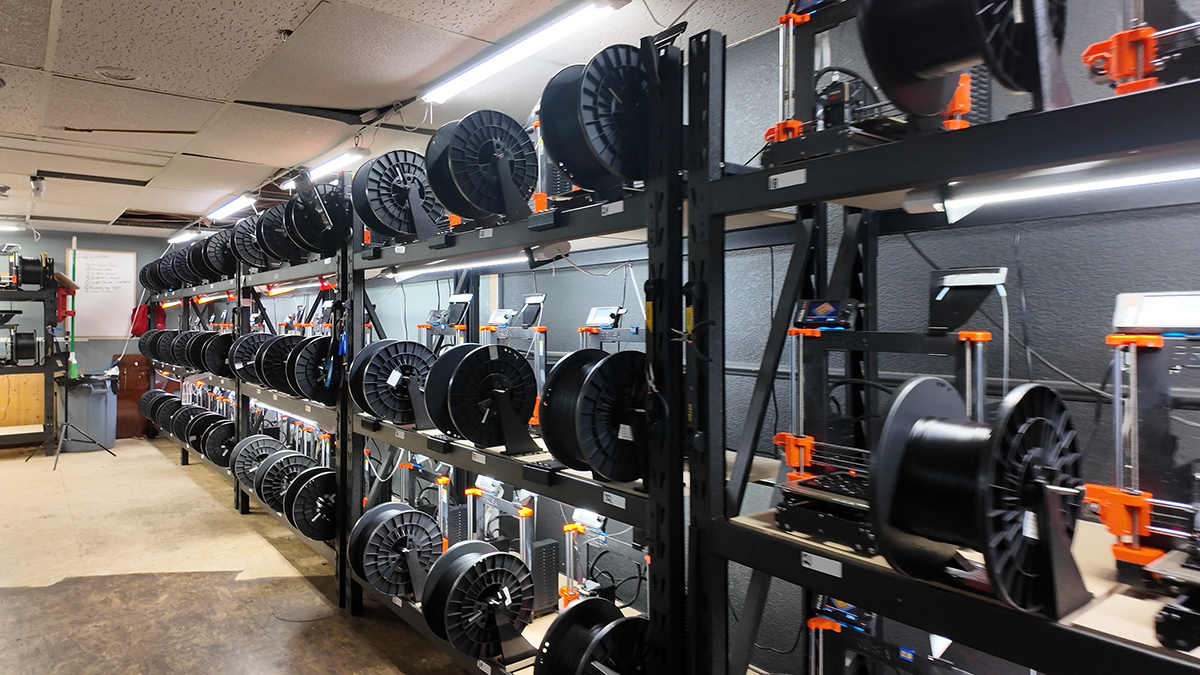
\includegraphics[width=\textwidth,keepaspectratio]{literature/3dprintfarm.jpg}
  \end{columns}
\end{frame}

% ── Slide 3: 9 hibaosztály ────────────────────────────────────────────────────
% All images from training_samples/ (correct orientation, consistent quality).
\begin{frame}{9 detektált hibaosztály}
  \centering
  \setlength{\tabcolsep}{5pt}
  \setlength{\fboxsep}{0pt}
  \setlength{\fboxrule}{0.4pt}
  \renewcommand{\arraystretch}{1.0}
  \begin{tabular}{ccc}
    \fbox{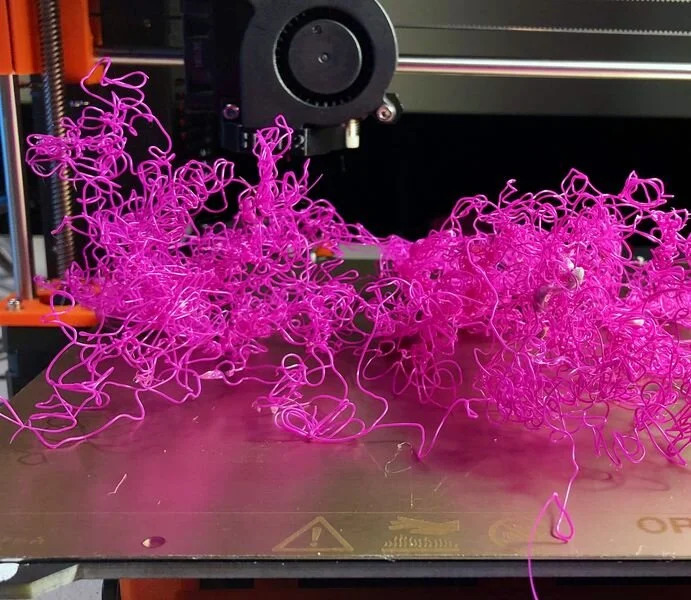
\includegraphics[width=2.9cm,height=1.7cm,keepaspectratio]{training_samples/spagetti.jpg}} &
    \fbox{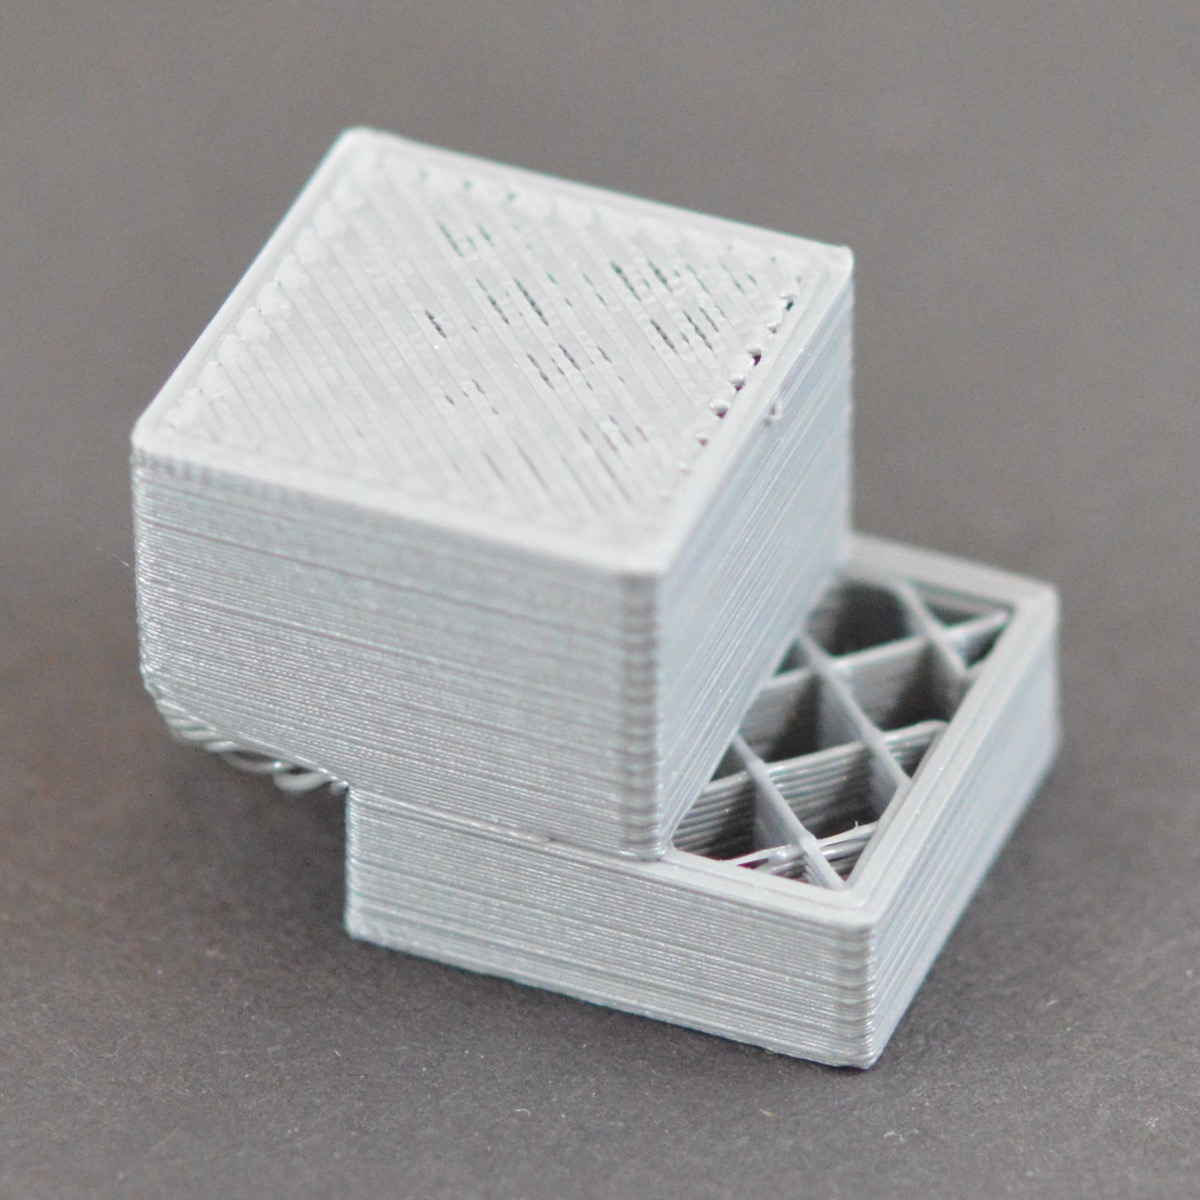
\includegraphics[width=2.9cm,height=1.7cm,keepaspectratio]{training_samples/layer_shift.jpg}} &
    \fbox{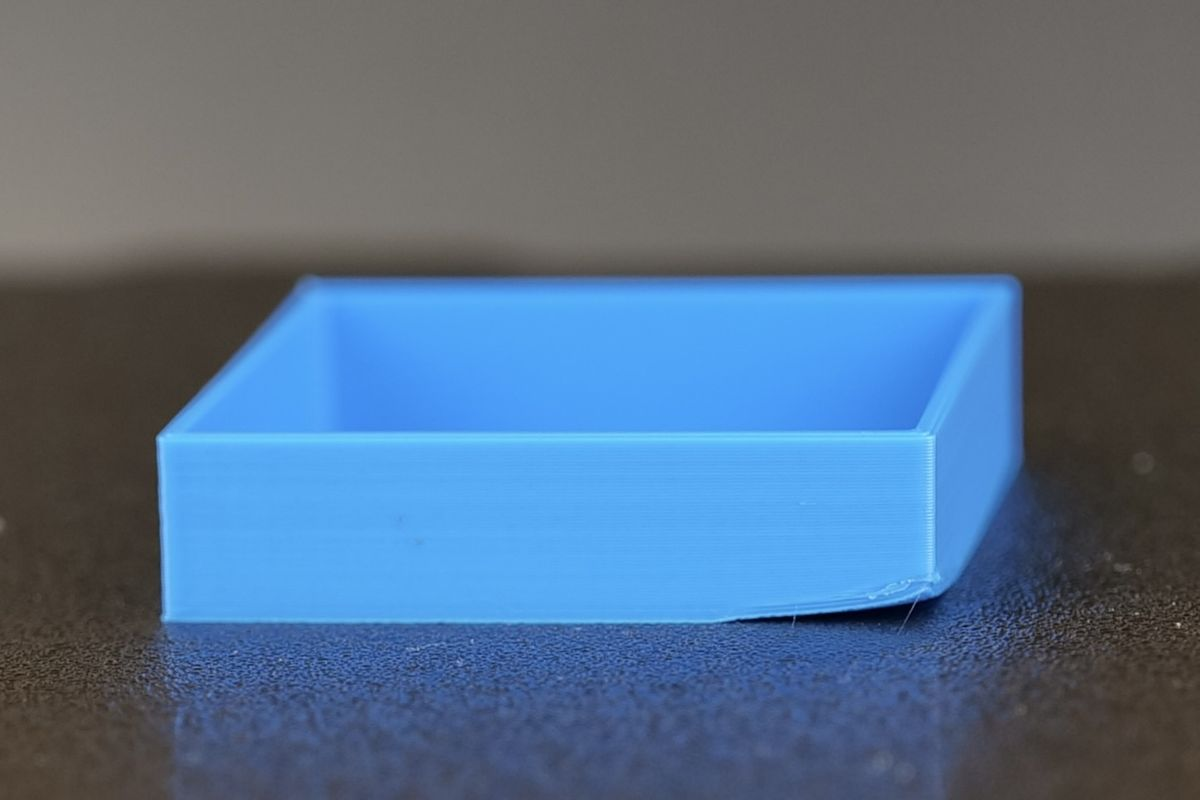
\includegraphics[width=2.9cm,height=1.7cm,keepaspectratio]{training_samples/warping.jpg}} \\[0.1em]
    {\scriptsize\textcolor{primary}{\textbf{spagetti}}} &
    {\scriptsize\textcolor{primary}{\textbf{réteg-eltolódás}}} &
    {\scriptsize\textcolor{primary}{\textbf{vetemedés}}} \\[0.3em]

    \fbox{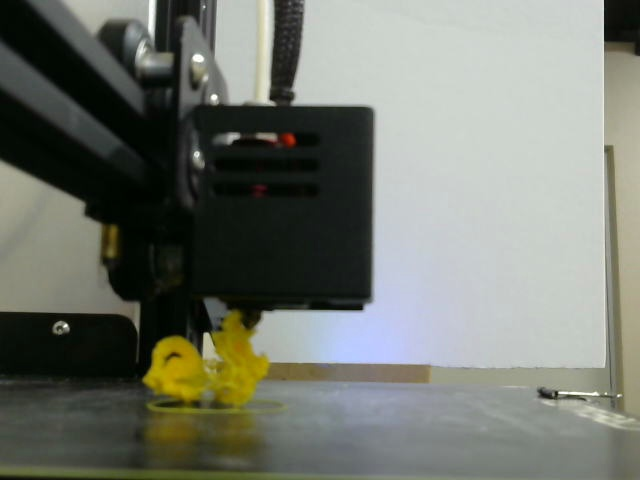
\includegraphics[width=2.9cm,height=1.7cm,keepaspectratio]{training_samples/not_sticking.jpg}} &
    \fbox{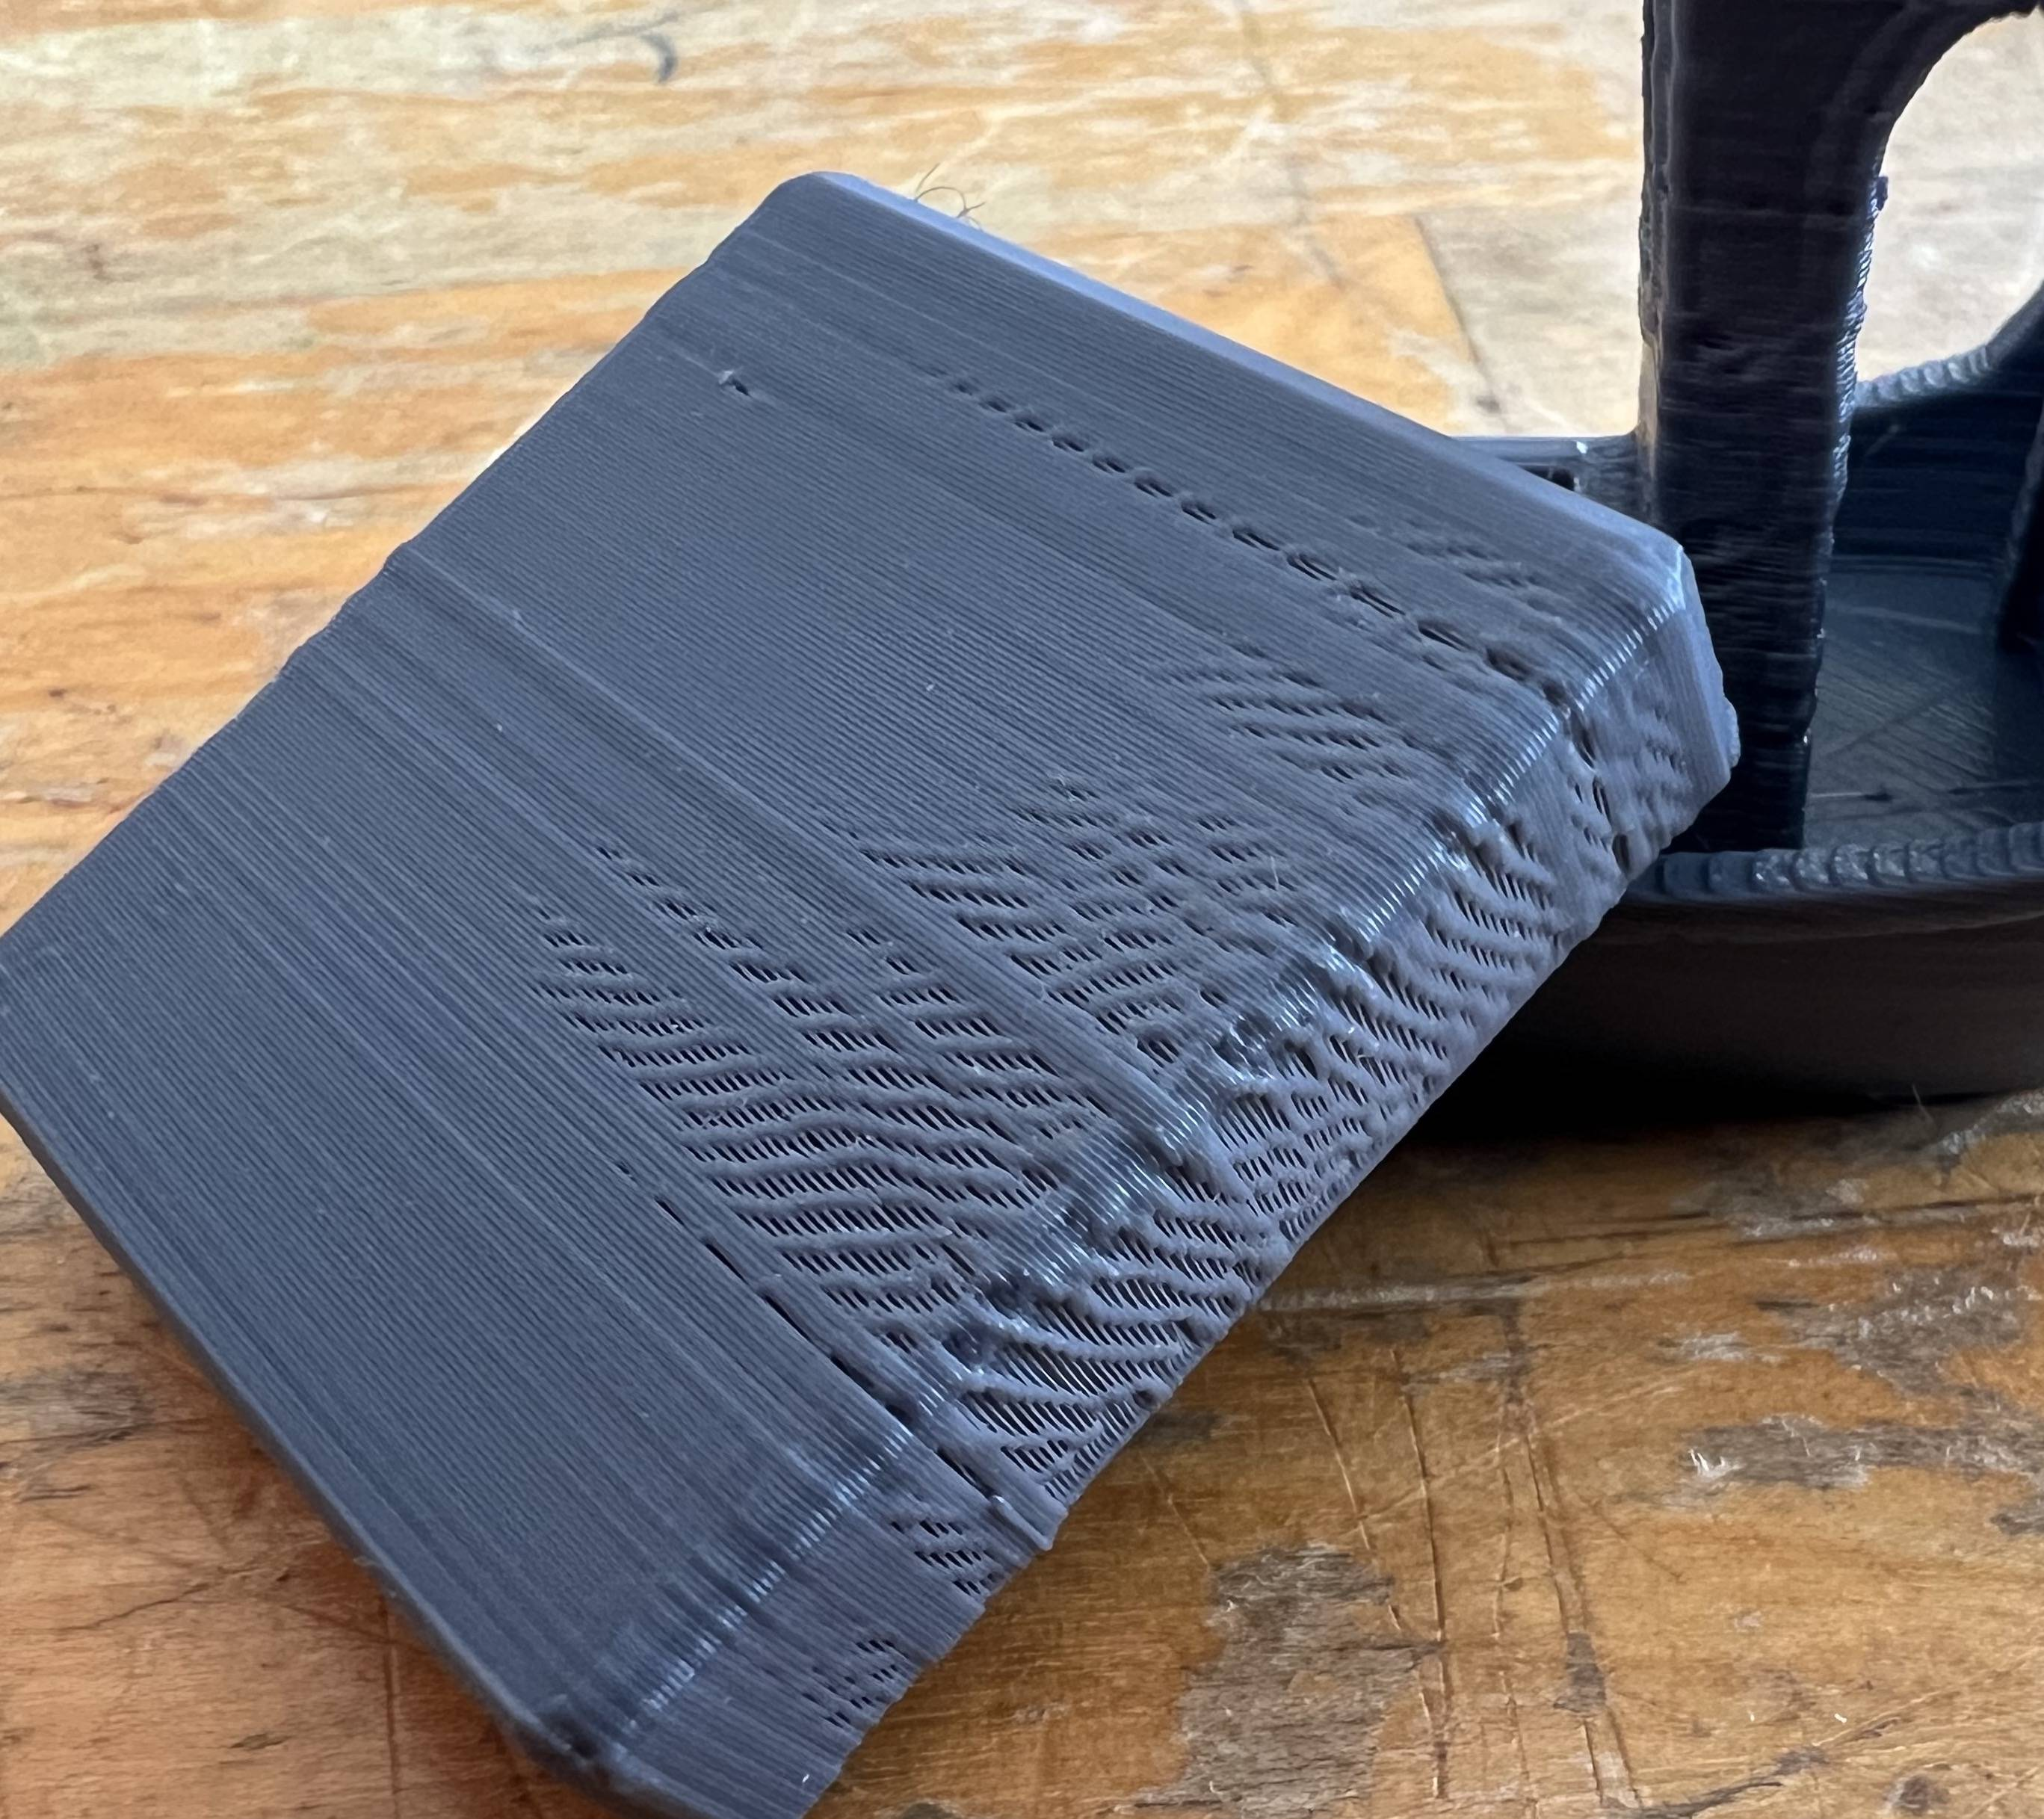
\includegraphics[width=2.9cm,height=1.7cm,keepaspectratio]{training_samples/under_extrusion.jpg}} &
    \fbox{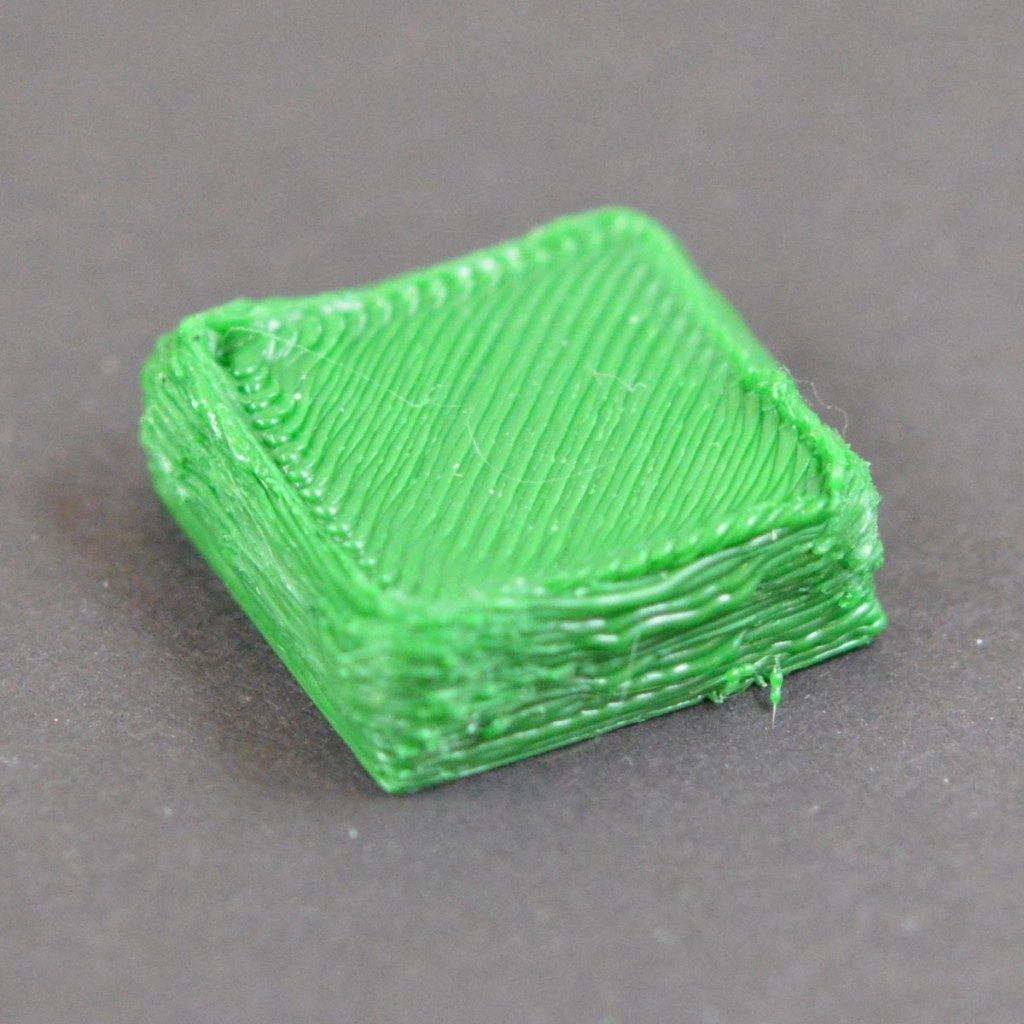
\includegraphics[width=2.9cm,height=1.7cm,keepaspectratio]{training_samples/over_extrusion.jpg}} \\[0.1em]
    {\scriptsize\textcolor{primary}{\textbf{nem tapadó réteg}}} &
    {\scriptsize\textcolor{primary}{\textbf{alul-extrúdálás}}} &
    {\scriptsize\textcolor{primary}{\textbf{felül-extrúdálás}}} \\[0.3em]

    \fbox{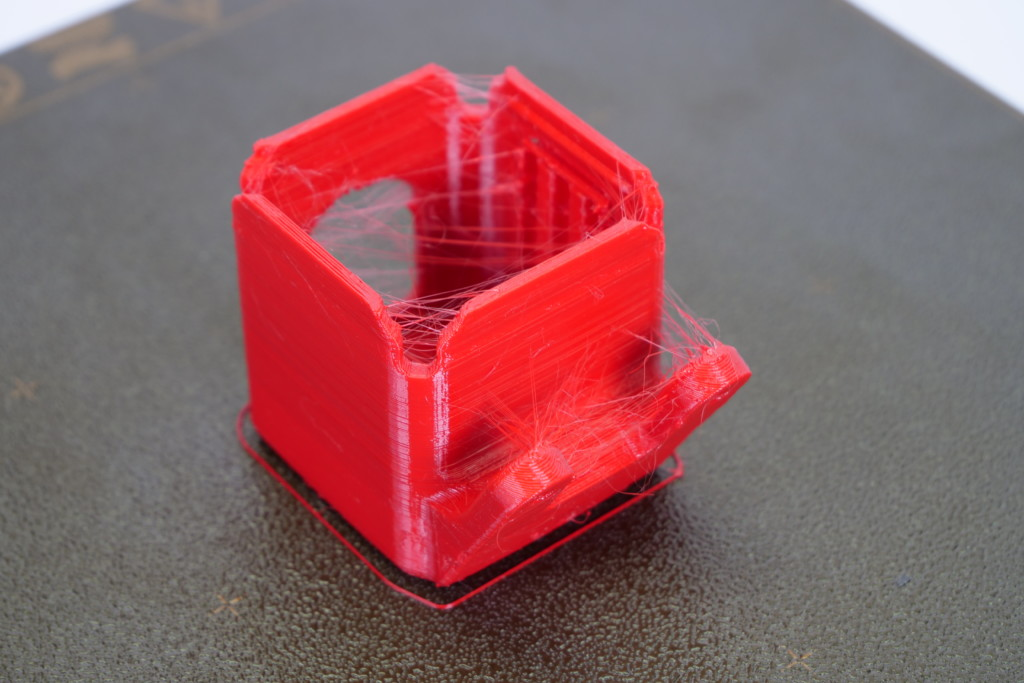
\includegraphics[width=2.9cm,height=1.7cm,keepaspectratio]{training_samples/stringing.jpg}} &
    \fbox{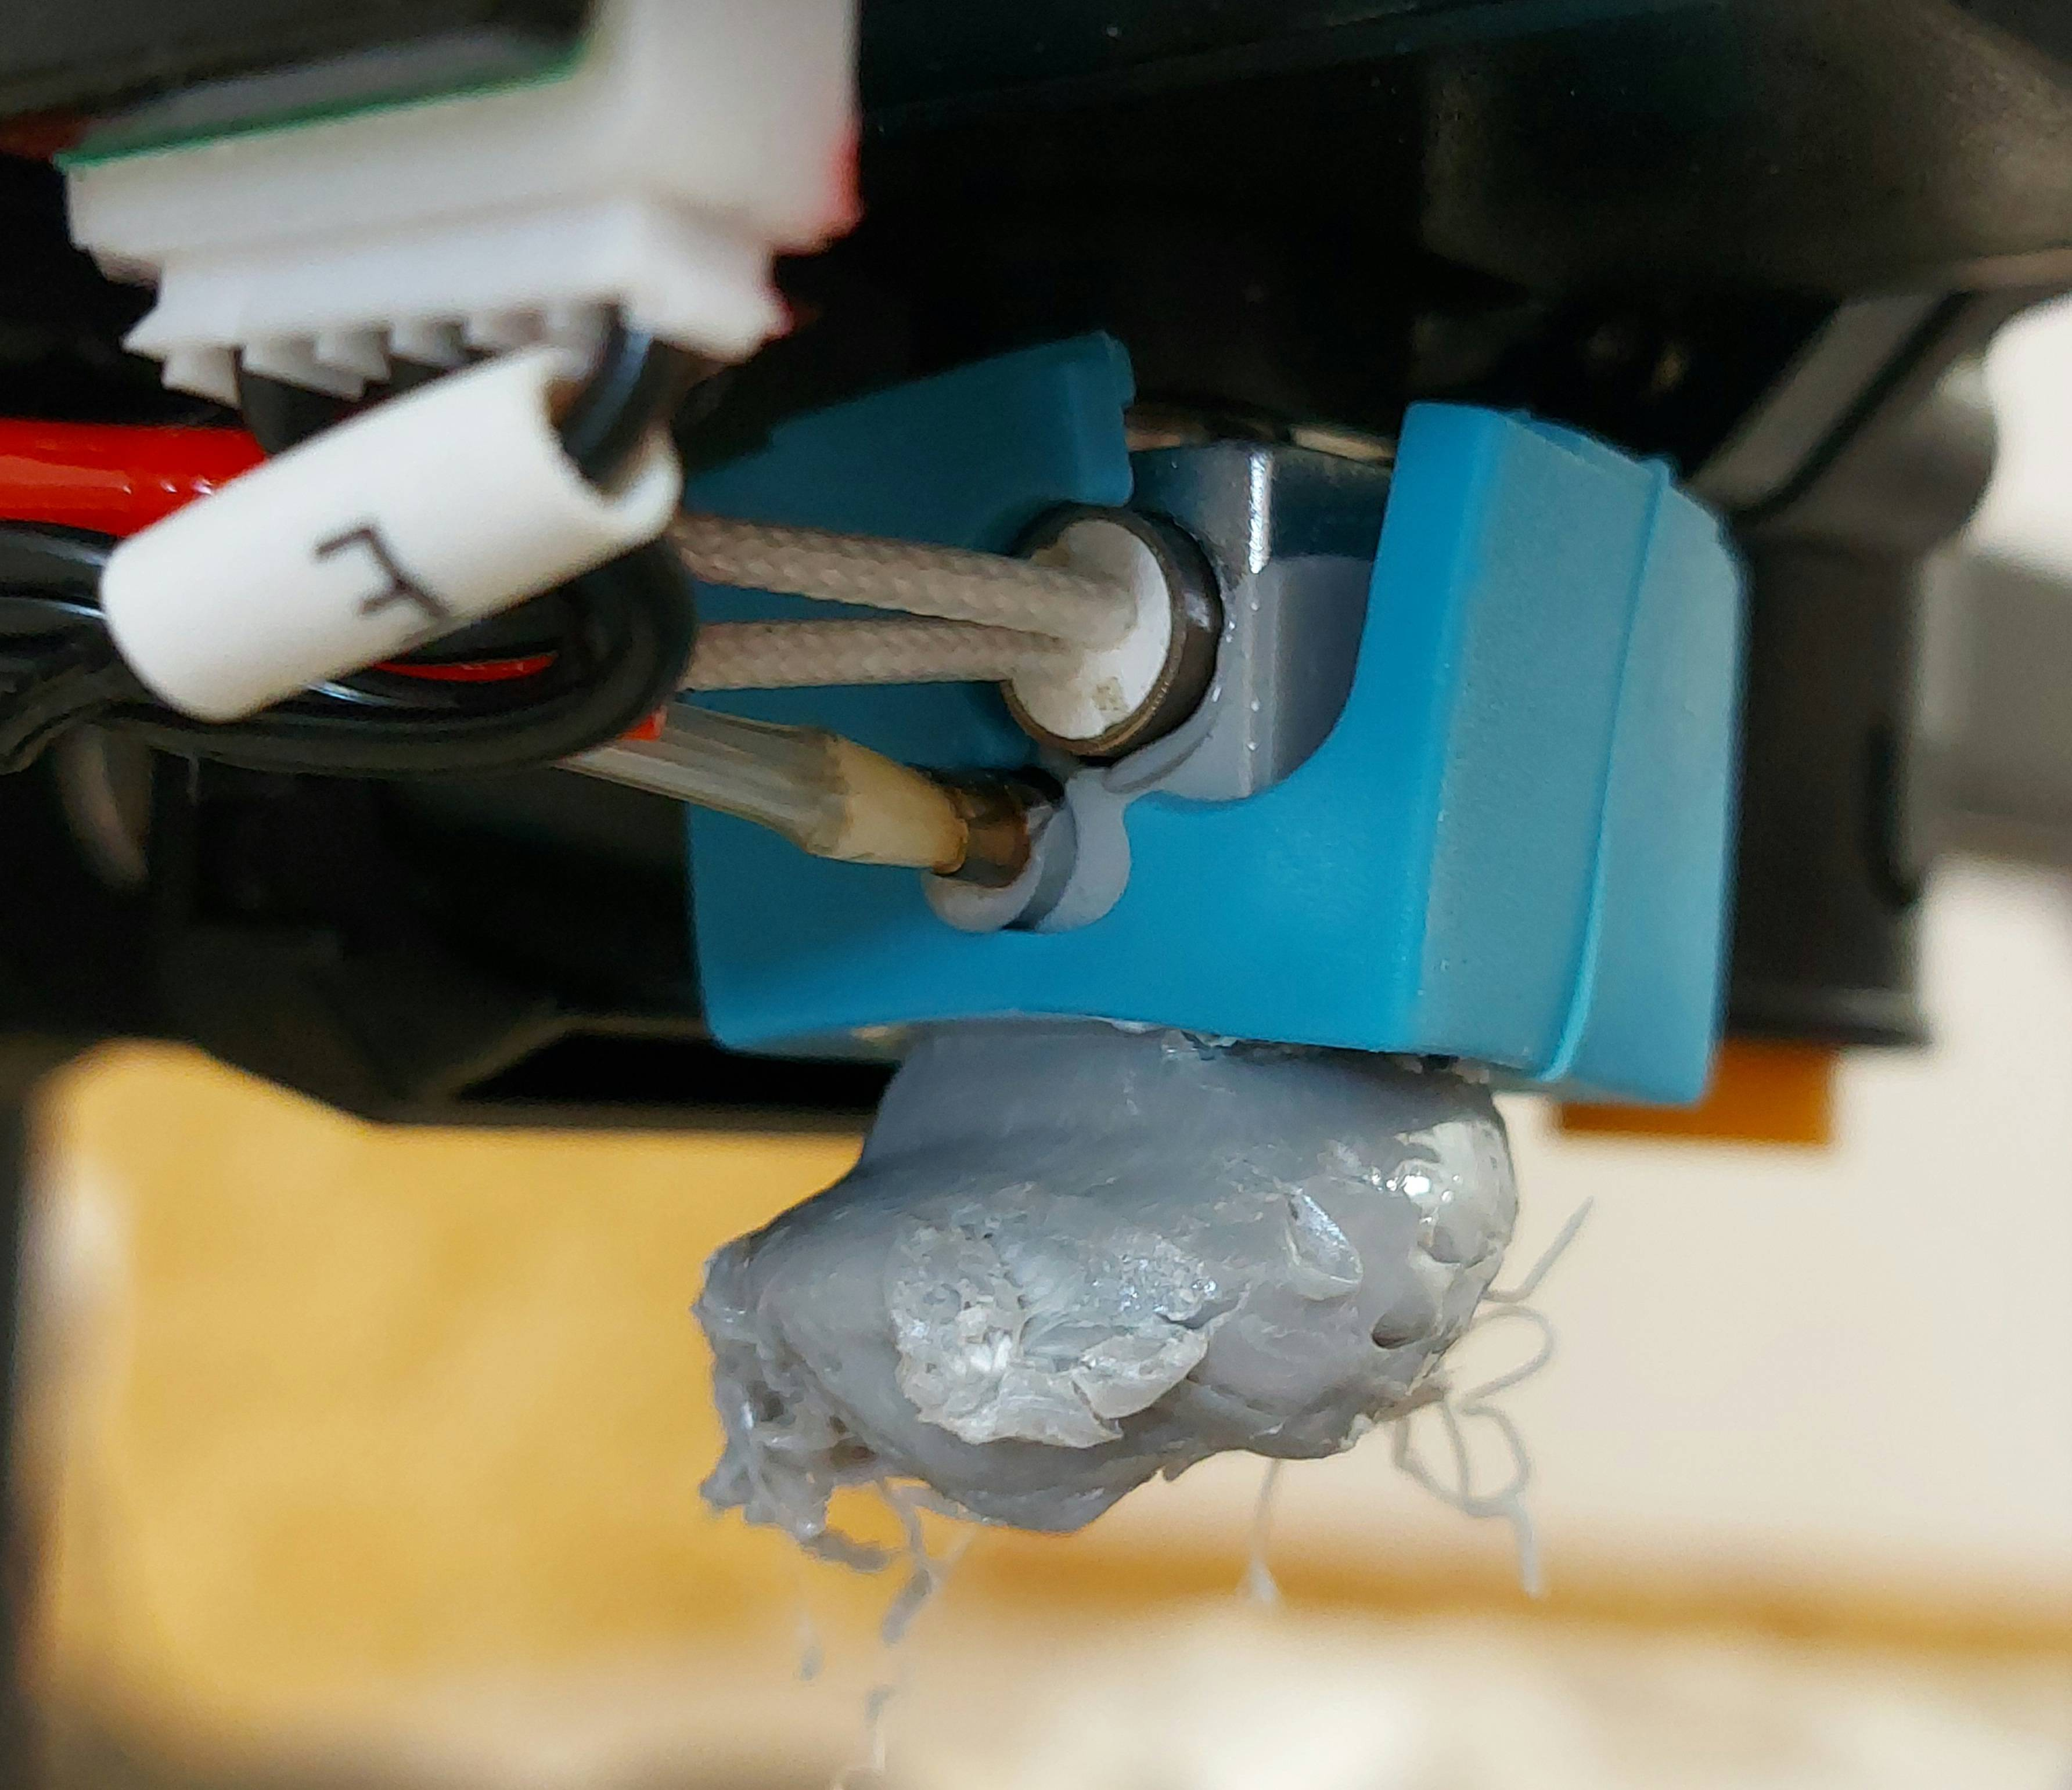
\includegraphics[width=2.9cm,height=1.7cm,keepaspectratio]{training_samples/nozzle_clog.jpg}} &
    \fbox{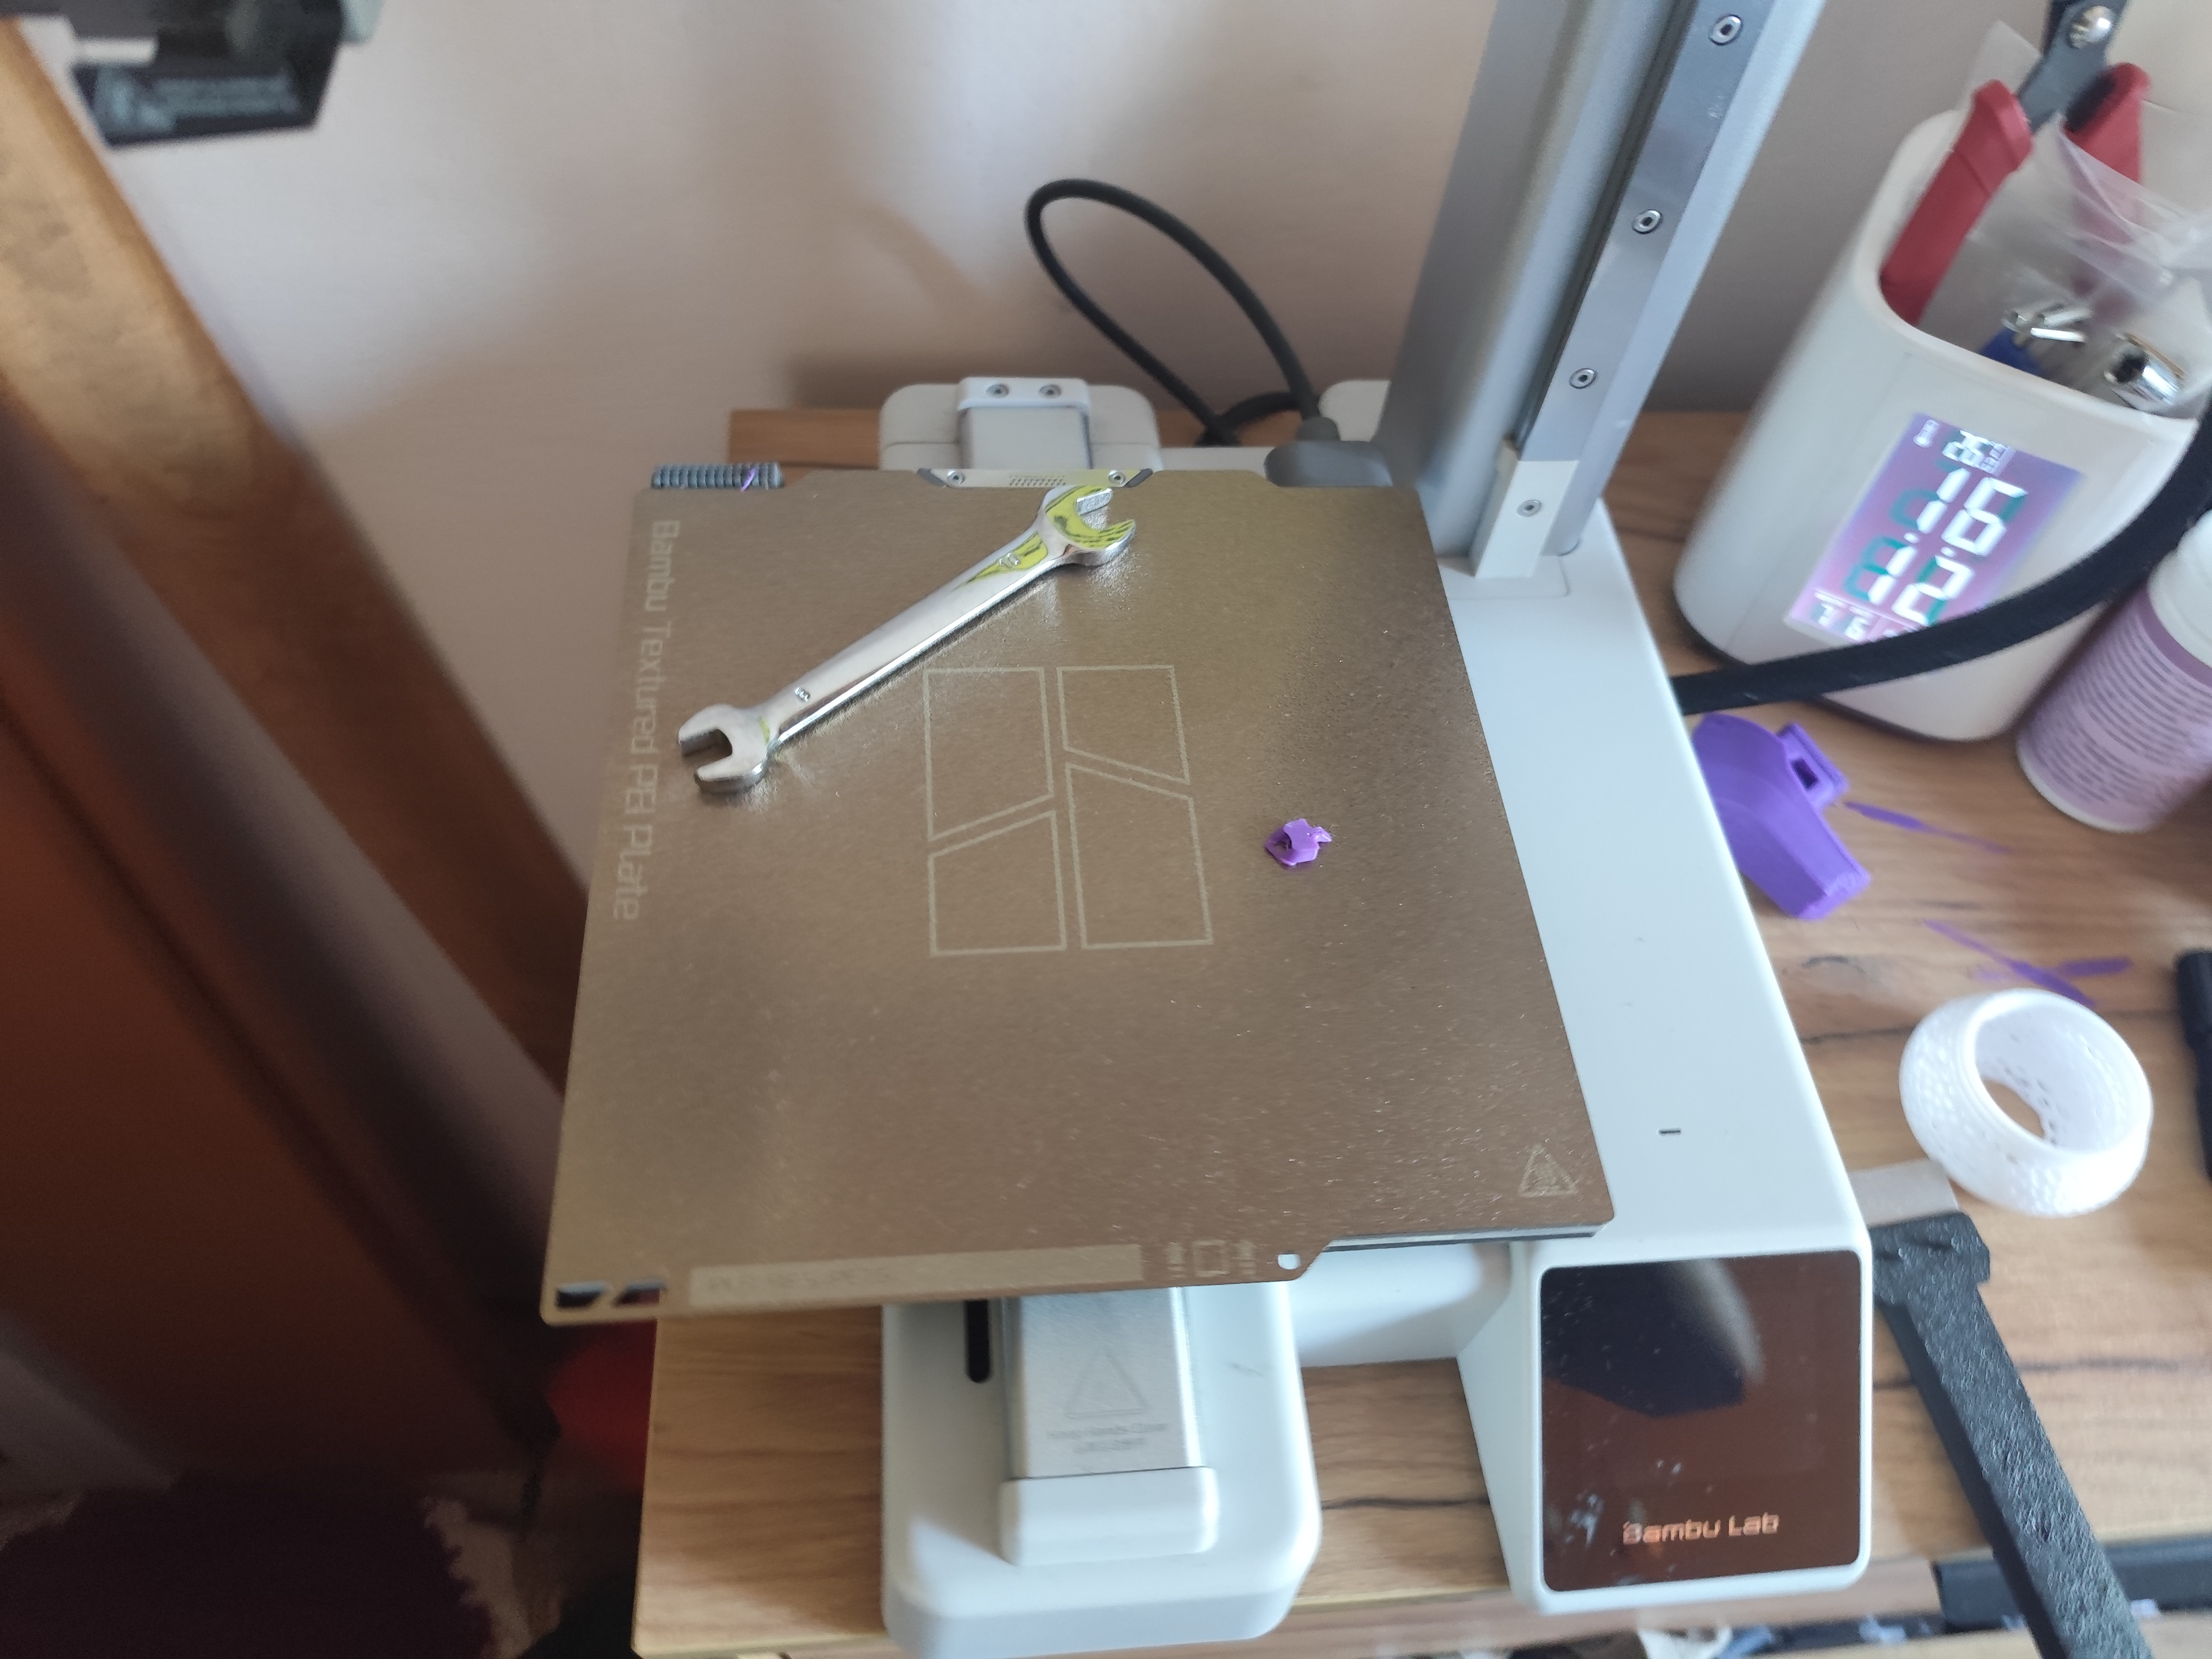
\includegraphics[width=2.9cm,height=1.7cm,keepaspectratio]{training_samples/foreign_object.jpg}} \\[0.1em]
    {\scriptsize\textcolor{primary}{\textbf{szálazás}}} &
    {\scriptsize\textcolor{primary}{\textbf{fúvóka-dugulás}}} &
    {\scriptsize\textcolor{primary}{\textbf{idegen tárgy}}}
  \end{tabular}
\end{frame}

% ── Slide 4: Adathalmaz ───────────────────────────────────────────────────────
\begin{frame}{Adathalmaz összeállítása}
  \begin{columns}[T]
    \column{0.54\textwidth}
      \textbf{\textcolor{primary}{Összesen: 2422 annotált kép · 9 osztály}}
      \vspace{0.4em}
      \begin{itemize}
        \setlength\itemsep{0.4em}
        \item Kaggle – Valenti \& Mikulhe adathalmazok
        \item HuggingFace – Javiai/failures-3D-print
        \item \textbf{397 saját felvétel} – projekt hardverén készült\\
              {\footnotesize(azonos kamerák, megvilágítás $\Rightarrow$ domain shift minimalizálása)}
        \item Annotálás: CVAT, bounding box formátum
        \item Felosztás: 80/20 train/val (seed = 42)
        \item Oversampling – alulreprezentált osztályokhoz
      \end{itemize}
    \column{0.44\textwidth}
      \begin{alertblock}{3-szintű augmentációs pipeline}
        \setlength\itemsep{0.3em}
        \begin{itemize}
          \item \textbf{Alaptranszf. (70\%):}\\
                tükrözés, fényerő, forgatás
          \item \textbf{Smart MixUp (20\%):}\\
                kompatibilis osztálypárok keverése
          \item \textbf{Mozaik (10\%):}\\
                4 kép $\rightarrow$ 1 vászon
        \end{itemize}
        \vspace{0.3em}
        \centering Tanítókészlet: \textbf{$\approx$4$\times$ bővülés}
      \end{alertblock}
    \end{columns}
\end{frame}

% ── Slide 5: YOLOv8x + kétfázisú tanítás ─────────────────────────────────────
\begin{frame}{YOLOv8x – Kétfázisú tanítási stratégia}
  \begin{columns}[T]
    \column{0.52\textwidth}
      \begin{block}{1. fázis – 960 px felbontás}
        \begin{itemize}
          \item Kiindulás: COCO előtanított súlyok
          \item Általános jellemzők megtanulása
        \end{itemize}
      \end{block}
      \vspace{0.4em}
      \begin{block}{2. fázis – 1280 px felbontás}
        \begin{itemize}
          \item Kiindulás: 1. fázis \texttt{best.pt}
          \item 100 epok · AdamW · koszinuszos LR
          \item Dropout: 0.1 · korai leállítás: 40 epok
          \item Erőteljes augmentáció (mosaic, mixup,\\copy-paste, RandAugment, erasing)
        \end{itemize}
      \end{block}
    \column{0.46\textwidth}
      \begin{alertblock}{Miért YOLOv8x?}
        \begin{itemize}
          \setlength\itemsep{0.3em}
          \item One-stage detektor – valós idejű inferencia
          \item Anchor-free architektúra
          \item Legjobb pontosság a YOLOv8 családban
          \item Inferencia a felhőben (T4 GPU) –\\nem az edge eszközön
        \end{itemize}
      \end{alertblock}
      \vspace{0.4em}
      \begin{exampleblock}{Konfidenciaküszöb}
        \centering 35\% – csúcs F1 $\approx$ 0.38-nál
      \end{exampleblock}
    \end{columns}
\end{frame}

% ── Slide 6: Tanítási görbék ──────────────────────────────────────────────────
\begin{frame}{Tanítási görbék – 100 epok}
  \centering
  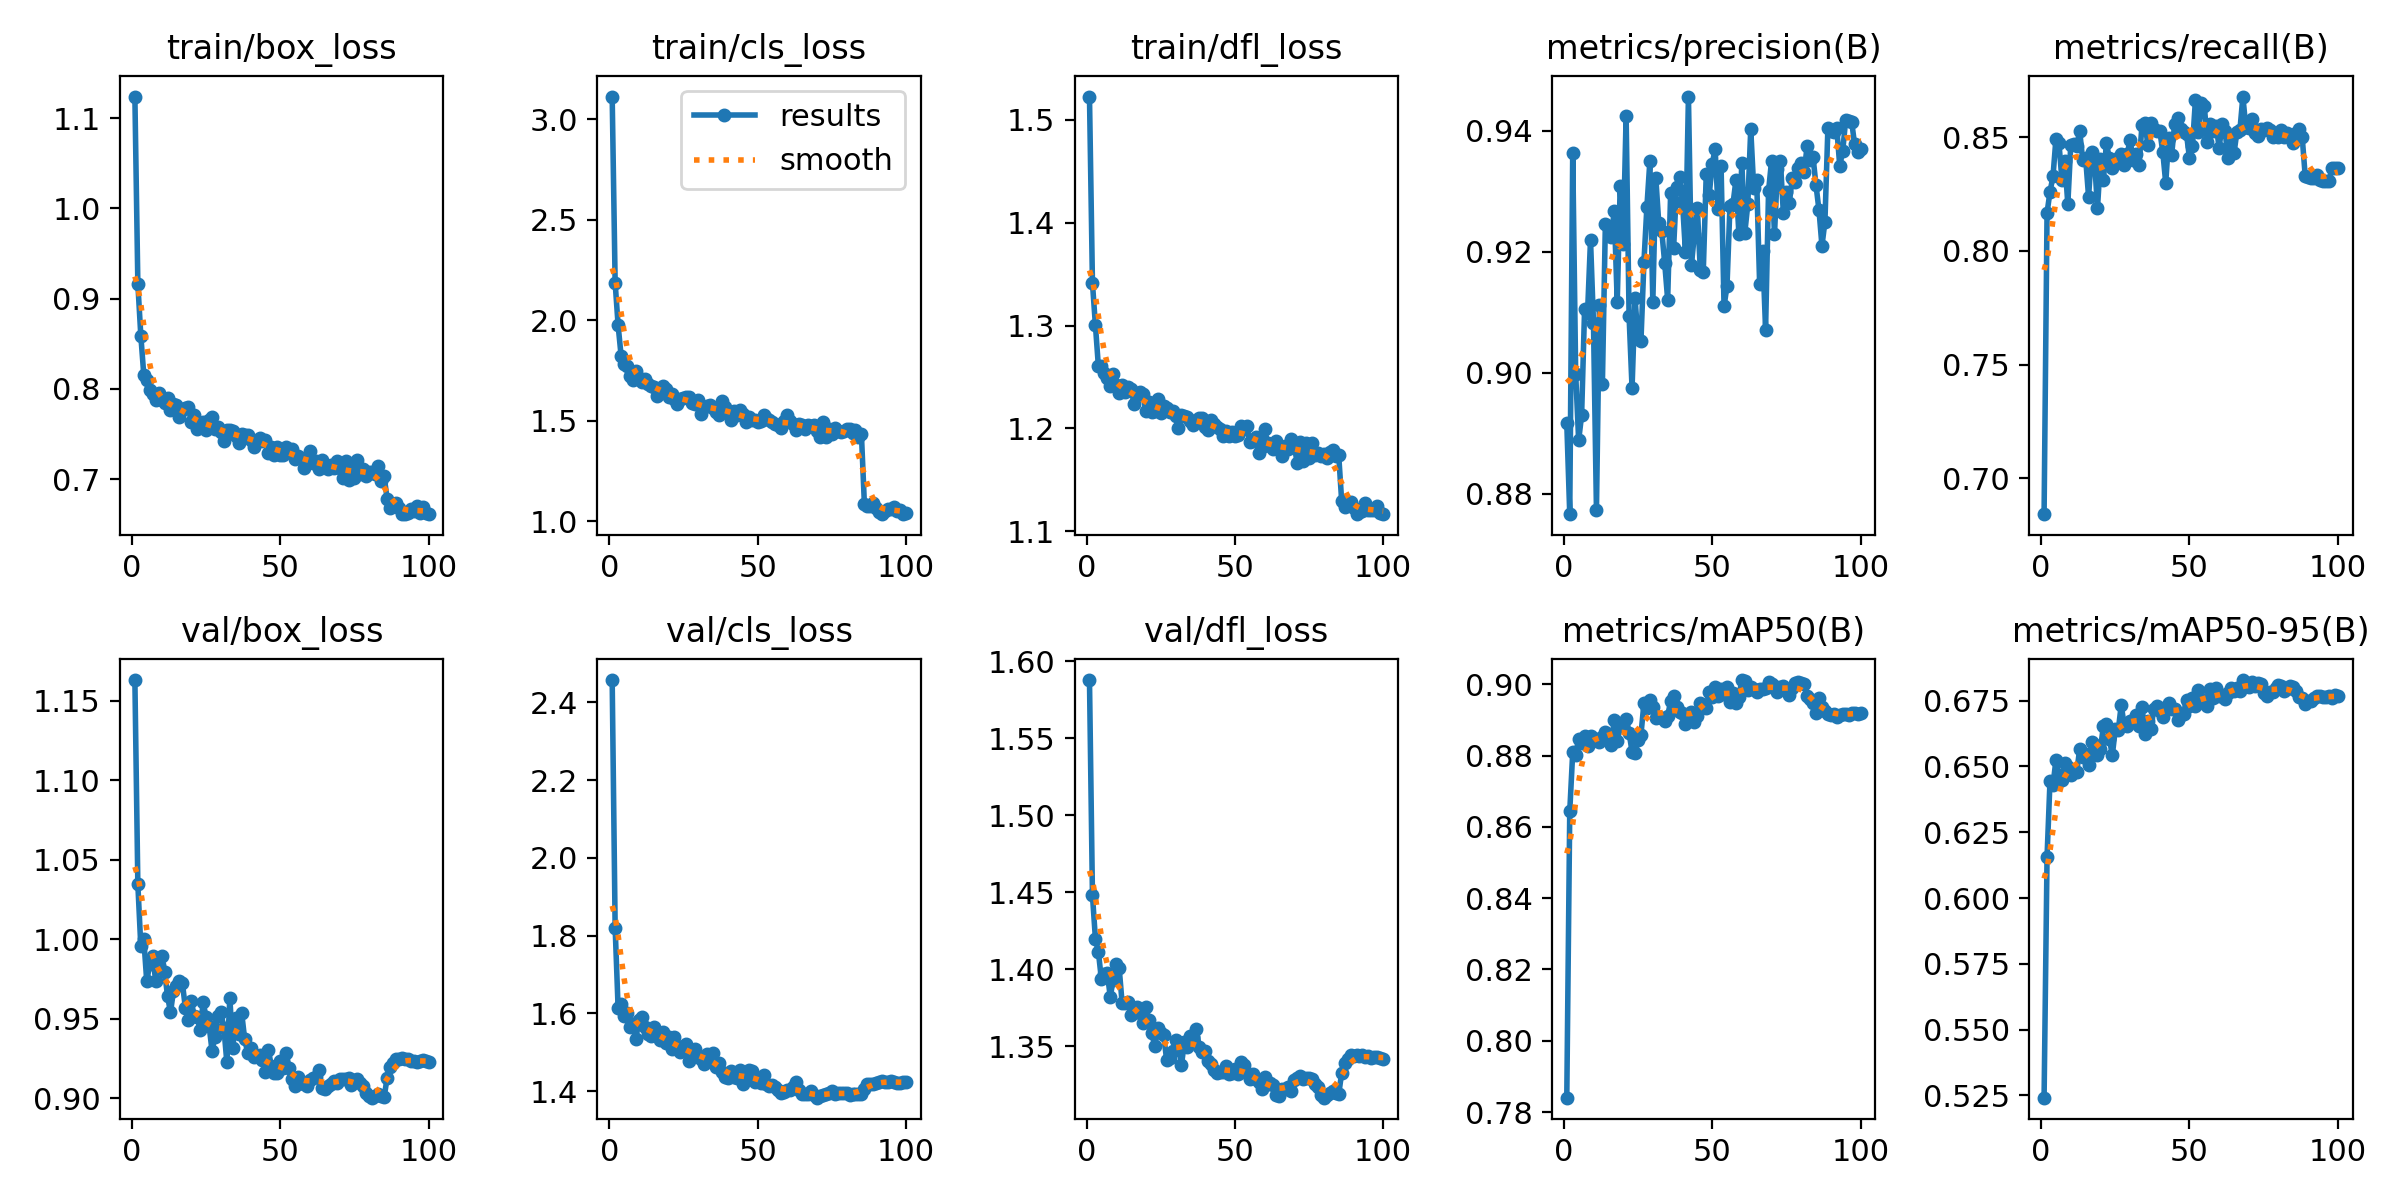
\includegraphics[width=0.88\textwidth,keepaspectratio]{results/y8x_phase2_12803/results.png}

  \vspace{0.25em}
  {\small
    Veszteségek stabilan csökkennek \quad
    mAP@0.5 csúcs: \textbf{0.901} (60. epok) \quad
    mAP@0.5:0.95 csúcs: \textbf{0.683} (68. epok)
  }
\end{frame}

% ── Slide 7: PR görbe + Konfúziós mátrix ─────────────────────────────────────
\begin{frame}{Precision-Recall görbe \& Konfúziós mátrix}
  \begin{columns}[c]
    \column{0.54\textwidth}
      \centering
      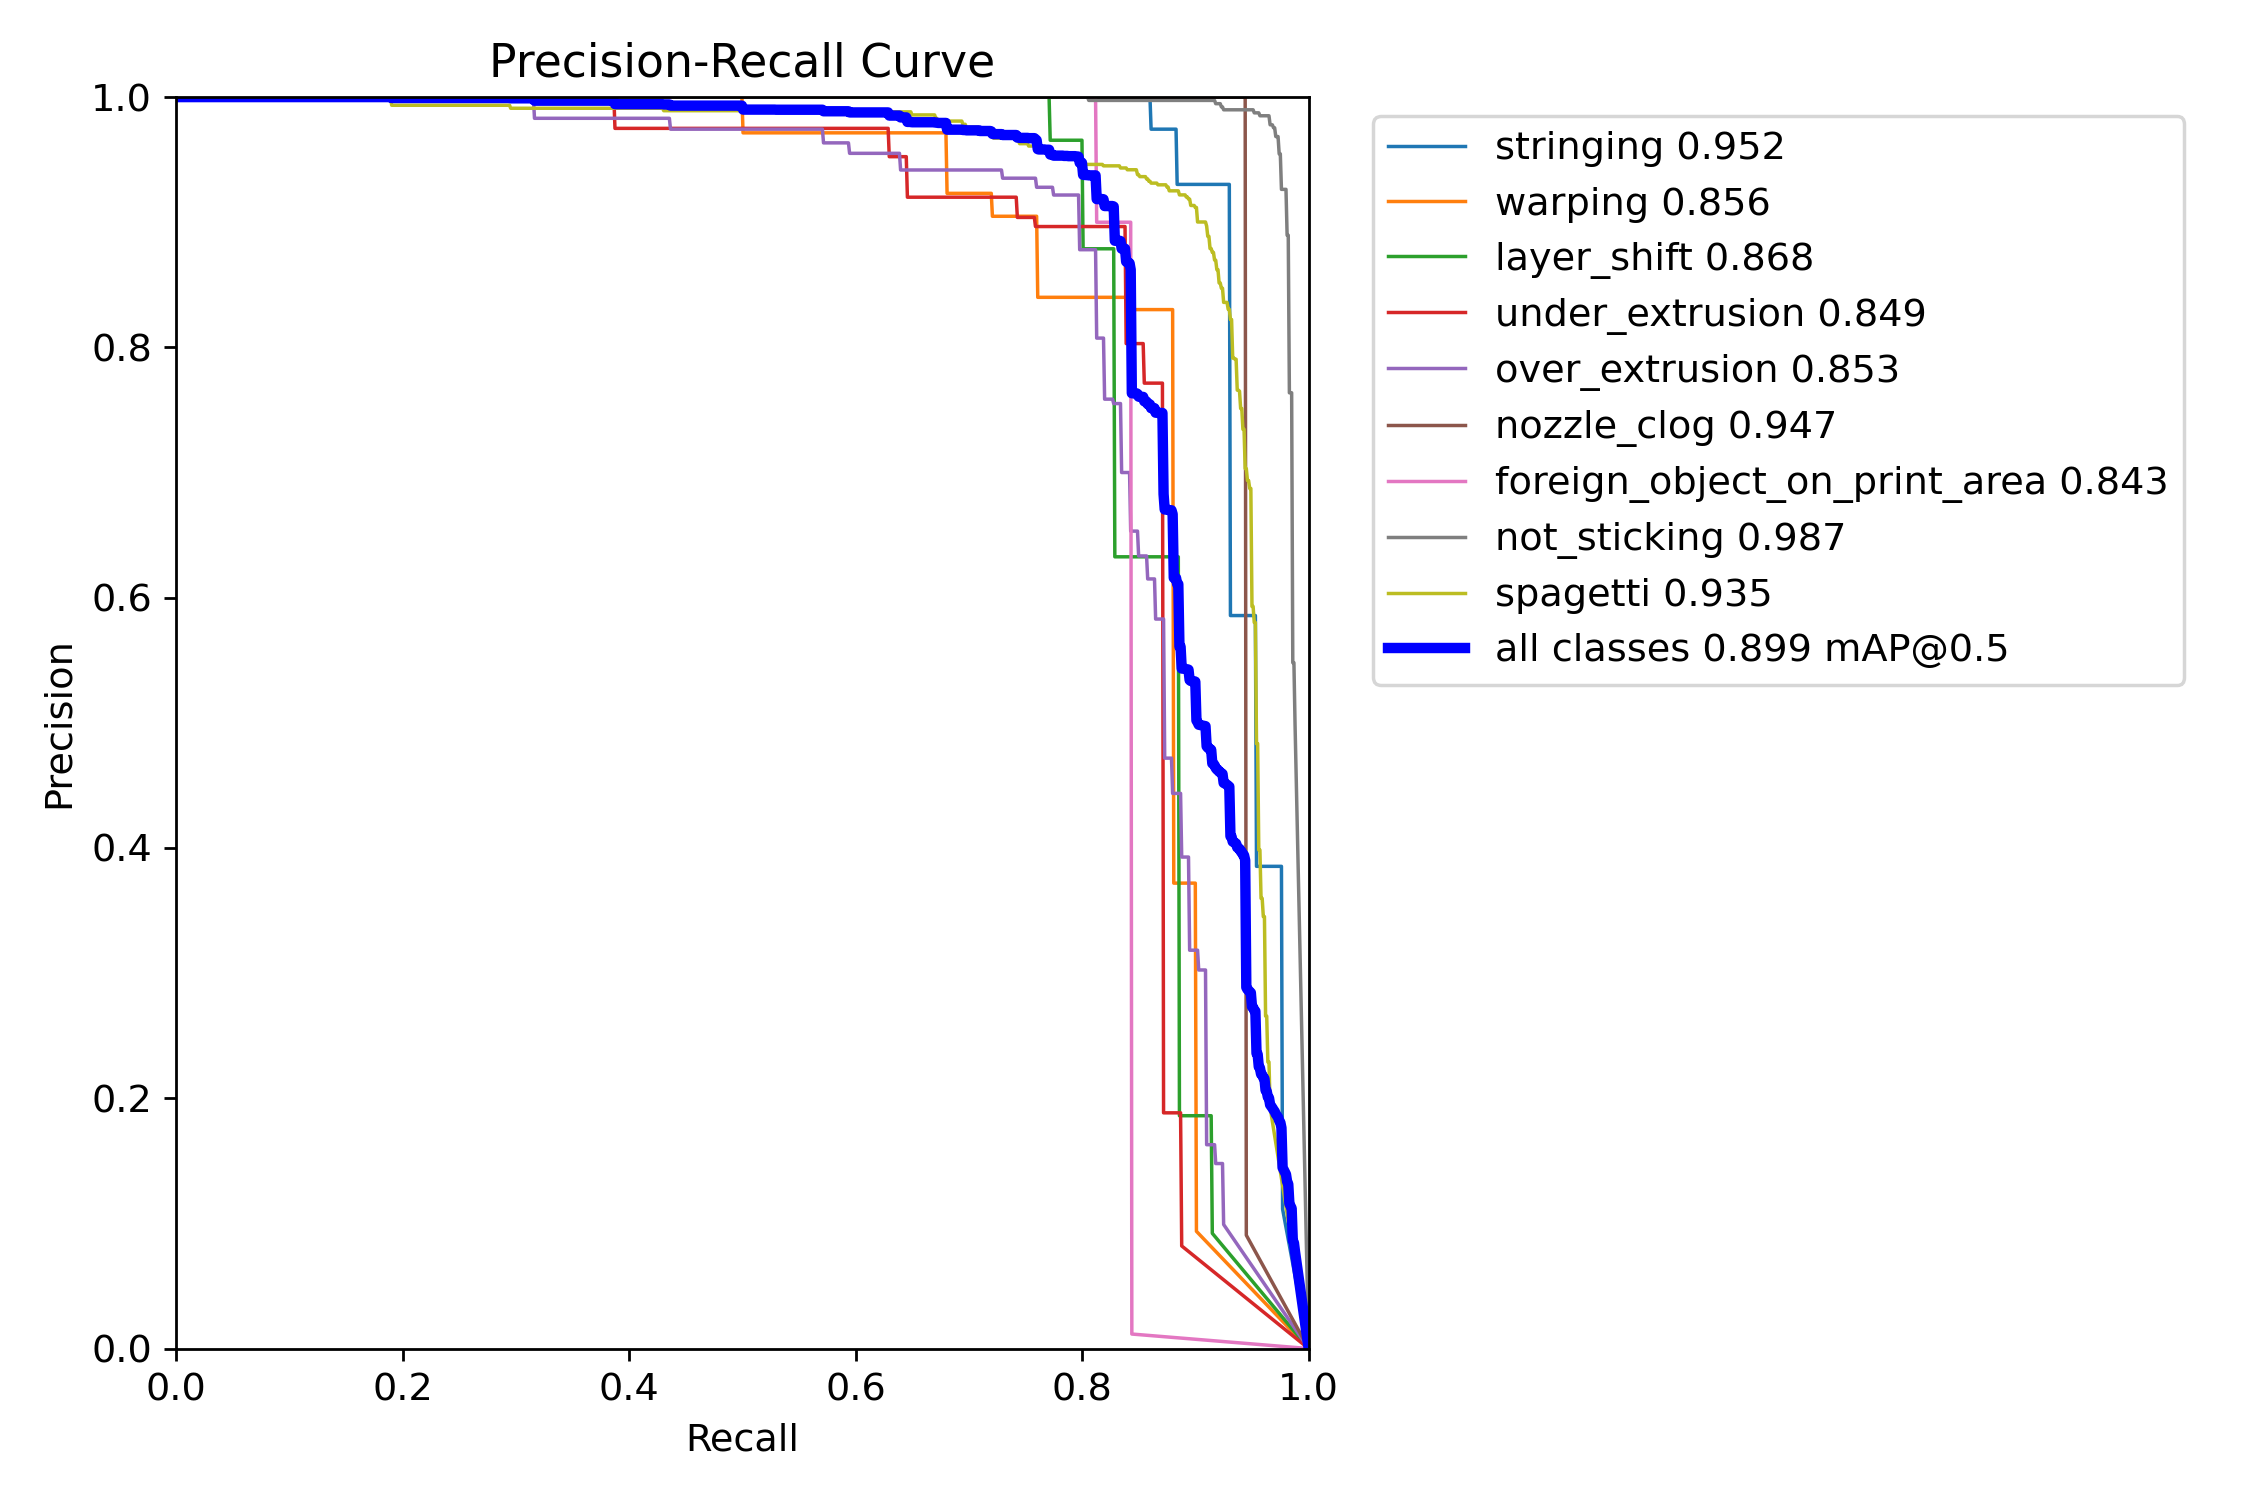
\includegraphics[width=\textwidth,keepaspectratio]{results/y8x_phase2_12803/BoxPR_curve.png}
    \column{0.44\textwidth}
      \centering
      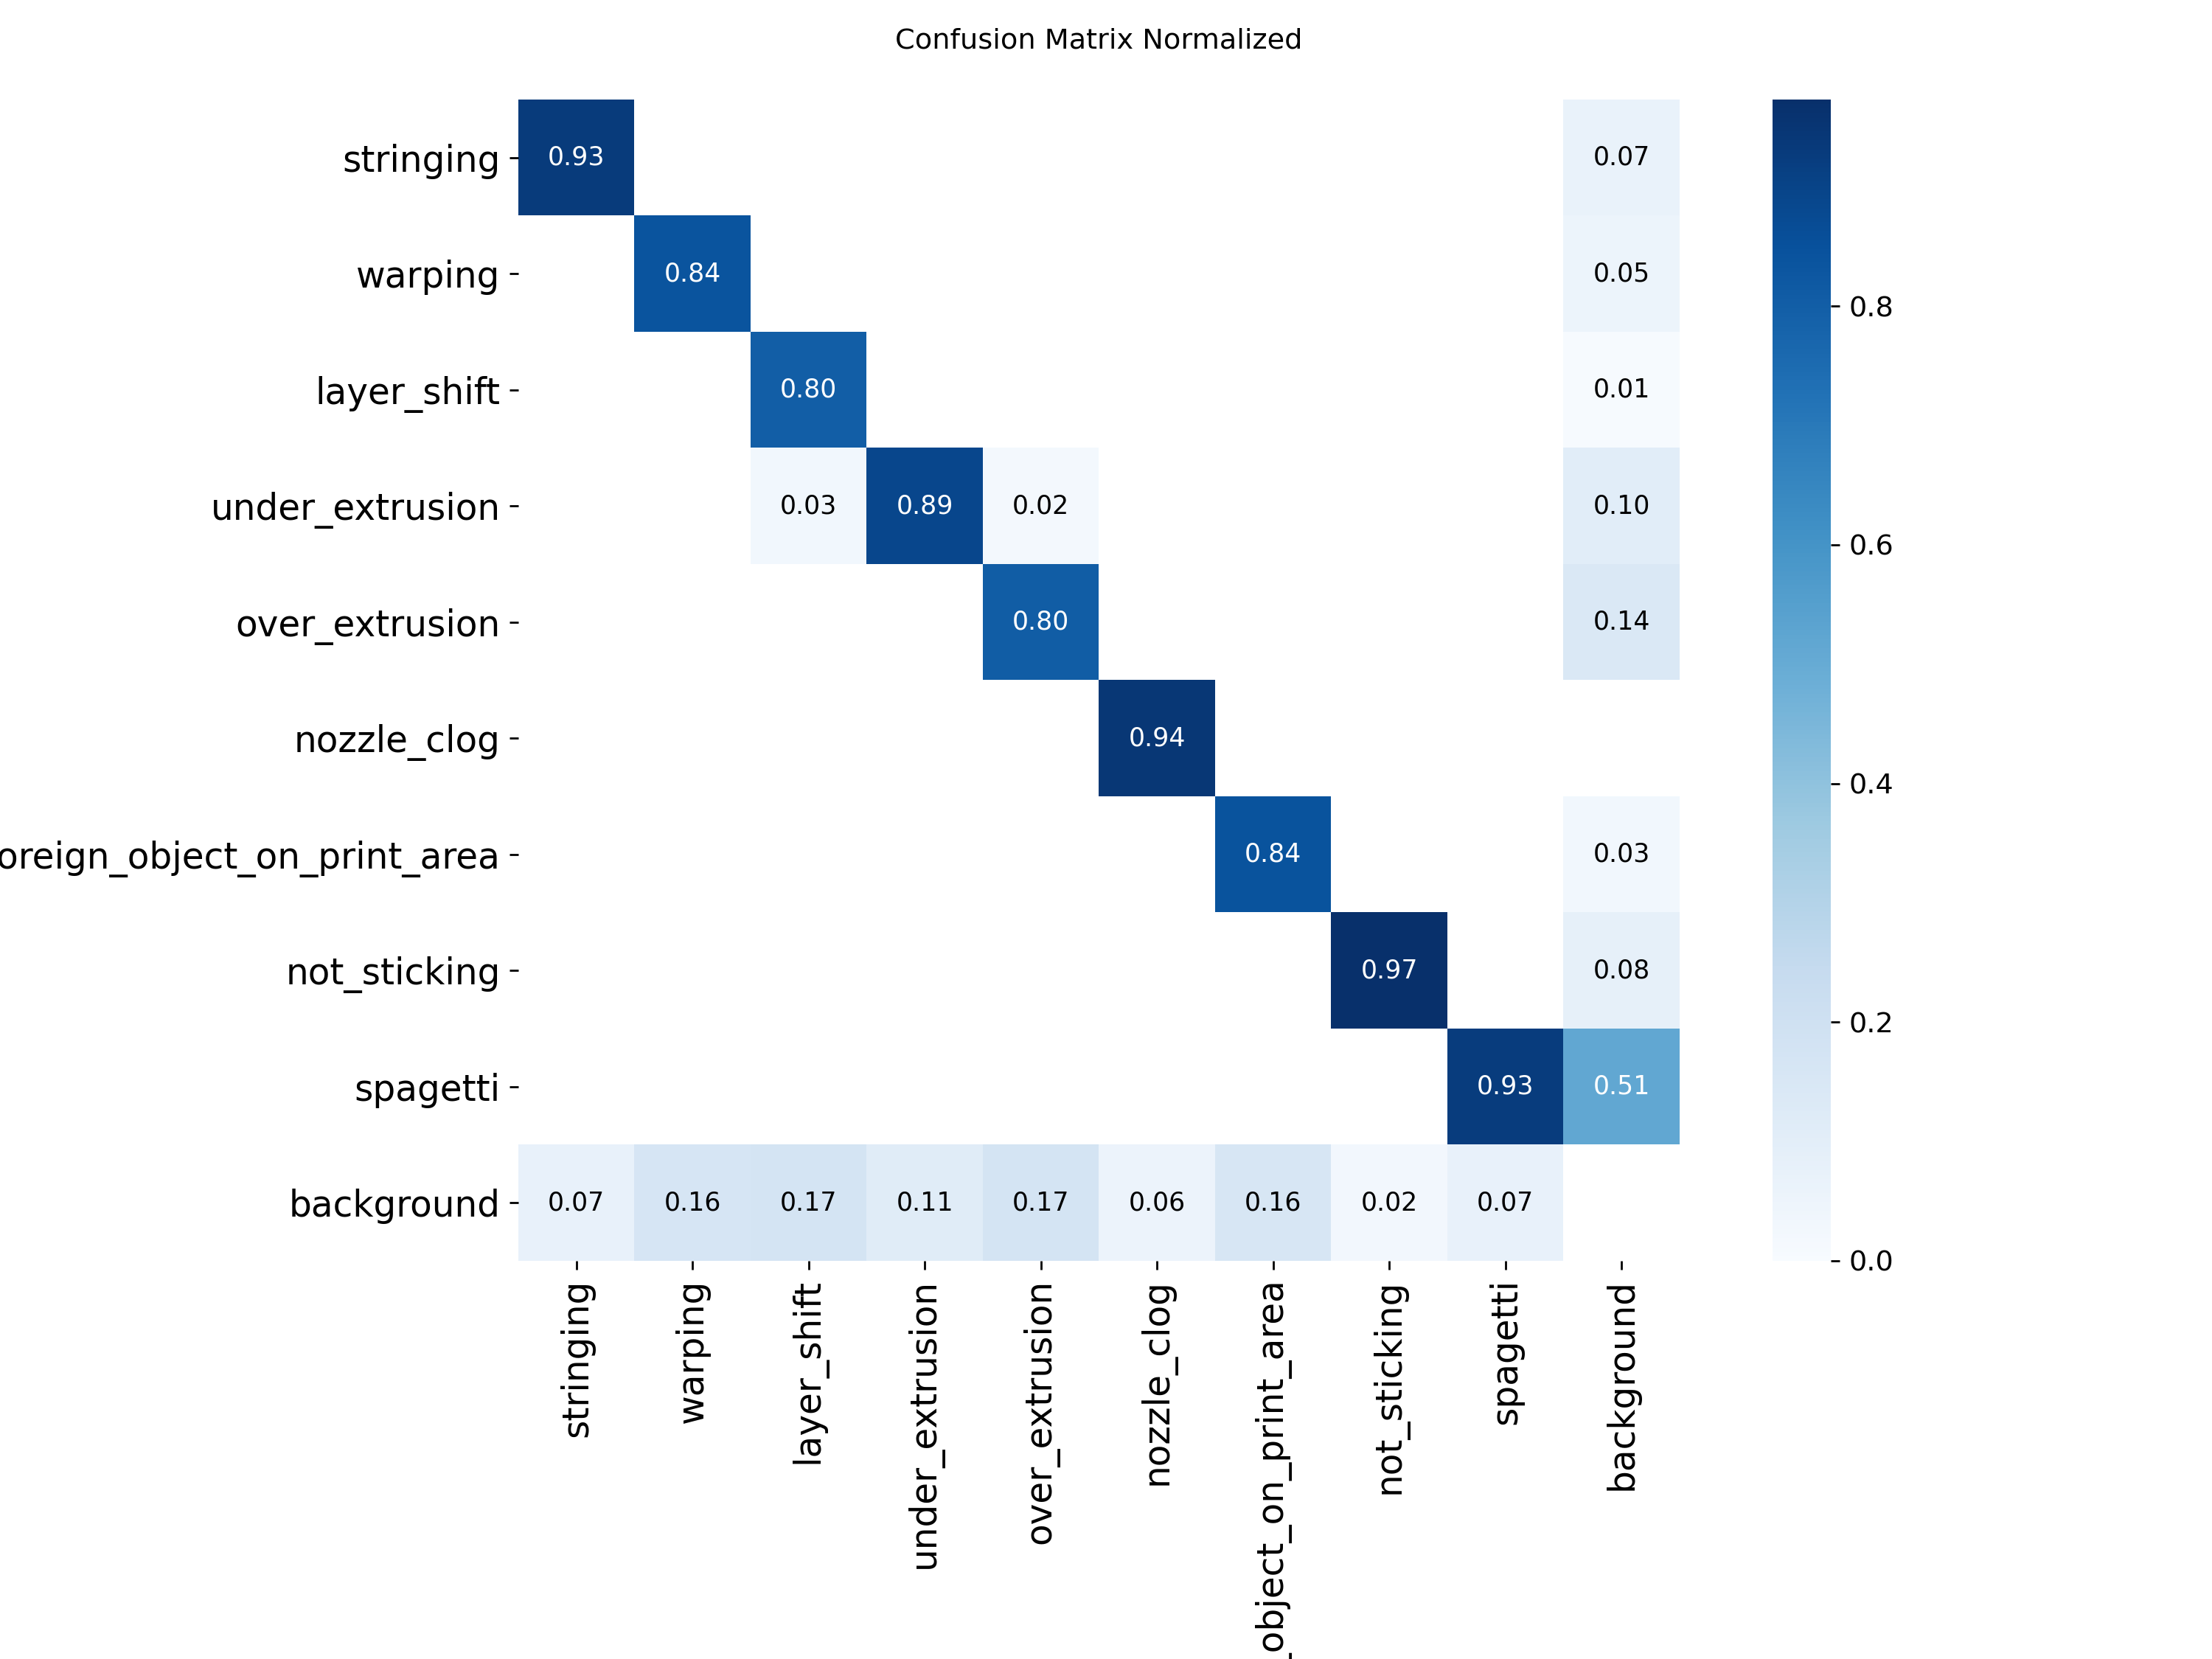
\includegraphics[width=\textwidth,keepaspectratio]{results/y8x_phase2_12803/confusion_matrix_normalized.png}
  \end{columns}
\end{frame}

% ── Slide 8: Validációs predikciók ────────────────────────────────────────────
\begin{frame}{Validációs predikciók – modell éles adatokon}
  \centering
  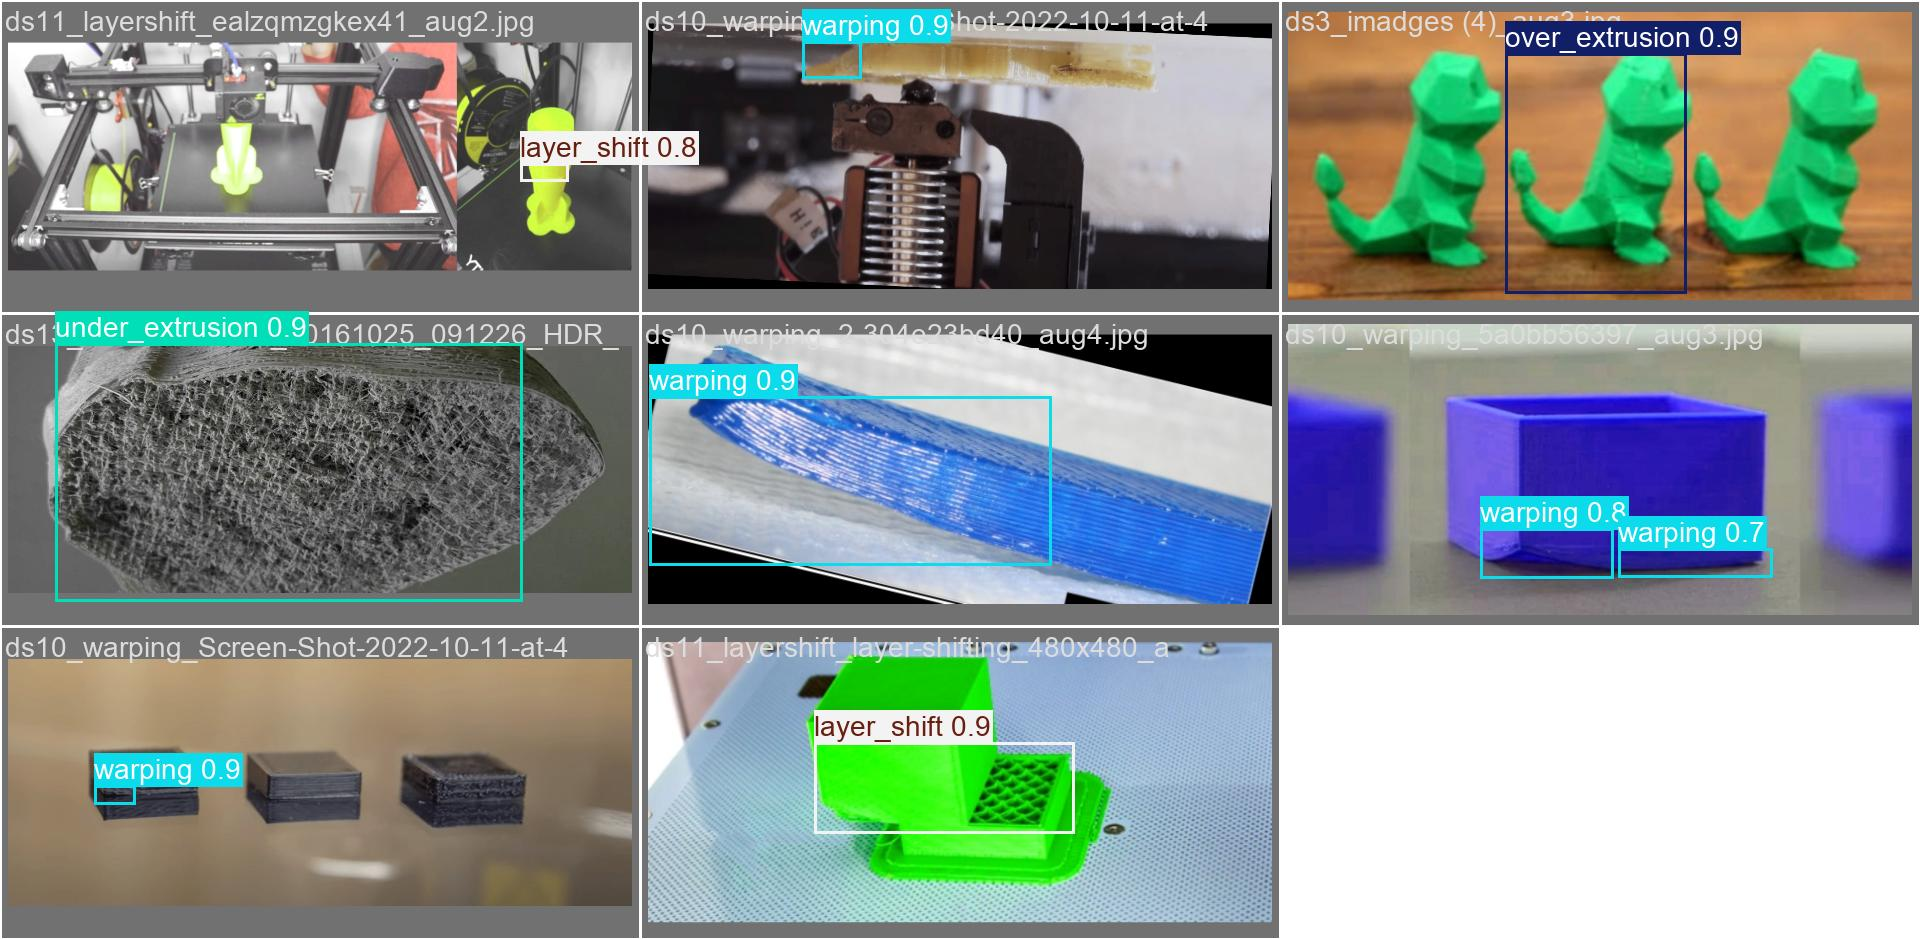
\includegraphics[width=0.90\textwidth,keepaspectratio]{results/y8x_phase2_12803/val_batch0_pred.jpg}

  \vspace{0.25em}
  {\small A bounding boxok pontosan illeszkednek a hibaterületekre, több hiba egyidejűleg is detektálható}
\end{frame}

% ── Slide 9: Összesített teljesítmény ────────────────────────────────────────
\begin{frame}{Összesített teljesítmény}
  \begin{columns}[c]
    \column{0.48\textwidth}
      \centering
      \renewcommand{\arraystretch}{1.45}
      \begin{tabular}{lc}
        \toprule
        \textbf{Metrika} & \textbf{Érték} \\
        \midrule
        Pontosság (Precision) & $0{,}937$ \\
        Visszahívás (Recall)  & $0{,}836$ \\
        mAP@0.5               & $0{,}892$ \\
        mAP@0.5:0.95          & $0{,}677$ \\
        \midrule
        Csúcs mAP@0.5         & $\mathbf{0{,}901}$ \\
        Csúcs F1              & $\mathbf{0{,}88}$ \\
        \bottomrule
      \end{tabular}
    \column{0.50\textwidth}
      \begin{block}{}
        \centering
        {\large $\mathbf{P = 0.937}$}\\[0.3em]
        {\small Szinte nulla hamis riasztás}
      \end{block}
      \vspace{0.4em}
      \begin{block}{}
        \centering
        {\large $\mathbf{R = 0.836}$}\\[0.3em]
        {\small A valós hibák 84\%-a detektálva}
      \end{block}
      \vspace{0.4em}
      \begin{exampleblock}{}
        \centering
        {\large $\mathbf{mAP@0.5 = 0.892}$}\\[0.3em]
        {\small 9 osztály · 1280 px · 2 fázis}
      \end{exampleblock}
  \end{columns}
\end{frame}

% ── Slide 10: Rendszerarchitektúra ────────────────────────────────────────────
\begin{frame}{Edge-Cloud hibrid architektúra}
  \centering
  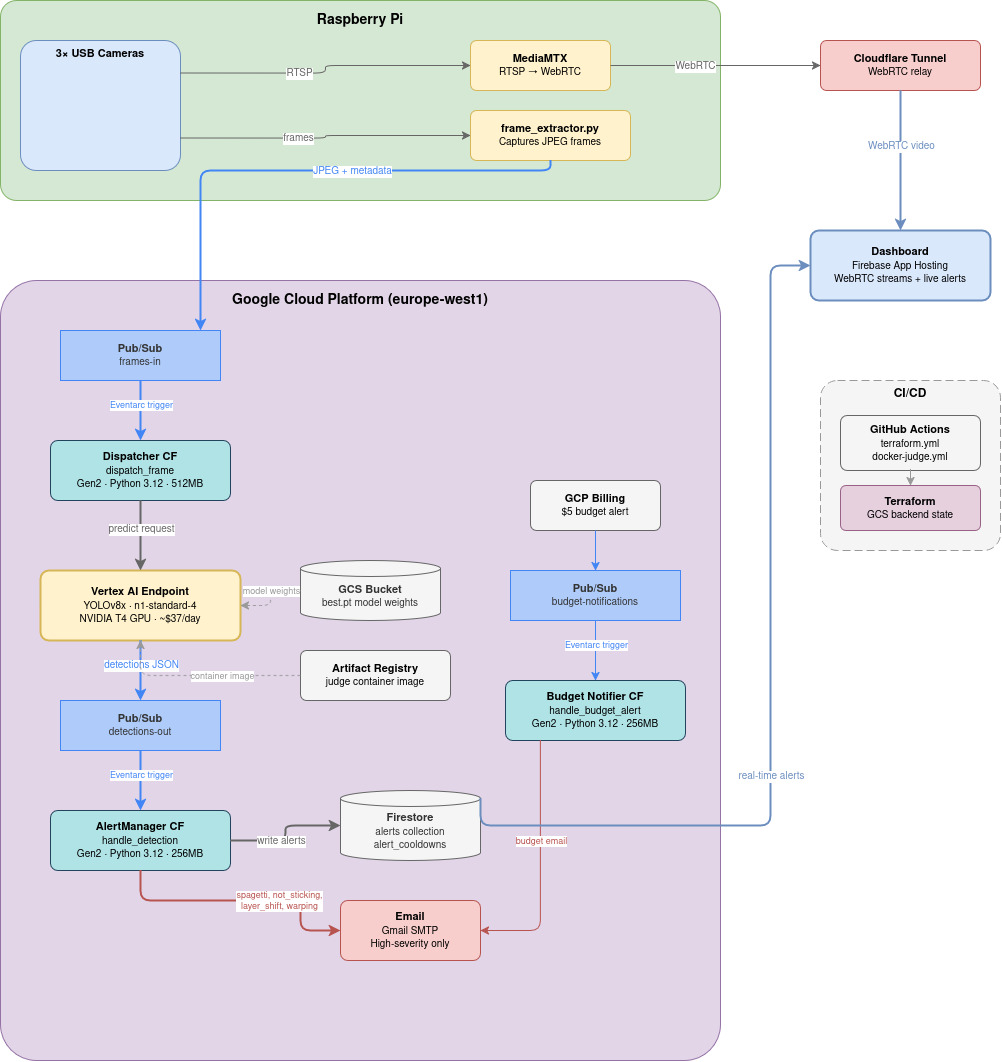
\includegraphics[width=0.90\textwidth,keepaspectratio]{literature/systemarch.jpg}
\end{frame}

% ── Slide 11: Adatfolyam ──────────────────────────────────────────────────────
\begin{frame}{Az adatfolyam lépései}
  \vspace{0.2em}
  \begin{enumerate}
    \setlength\itemsep{0.45em}
    \item \textbf{Raspberry Pi 4B} (3 webkamera) $\rightarrow$ \texttt{frame-extractor}:\\
          2 fps/kamera, 640×480 JPEG $\rightarrow$ Pub/Sub \texttt{frames-in}
    \item \textbf{Dispatcher} Cloud Function $\rightarrow$ Vertex AI \texttt{/predict}
          (OAuth2 hitelesítés)
    \item \textbf{Judge} konténer (YOLOv8x, T4 GPU) $\rightarrow$
          Pub/Sub \texttt{detections-out}
    \item \textbf{Alert-Manager}: Firestore + HTML e-mail
          {\footnotesize(60 s cooldown / kamera, csak magas súlyosságú hibáknál)}
    \item \textbf{Dashboard}: Firestore \texttt{onSnapshot} + WebRTC stream
          (Cloudflare alagút)
  \end{enumerate}

  \vspace{0.5em}
  \begin{block}{\small Infrastruktúra \& CI/CD}
    \small Terraform (IaC) \quad GitHub Actions (3 workflow) \quad Checkov biztonsági scan
  \end{block}
\end{frame}

% ── Slide 12: Dashboard ───────────────────────────────────────────────────────
\begin{frame}{Élő dashboard}
  \begin{columns}[c]
    \column{0.5\textwidth}
      \centering
      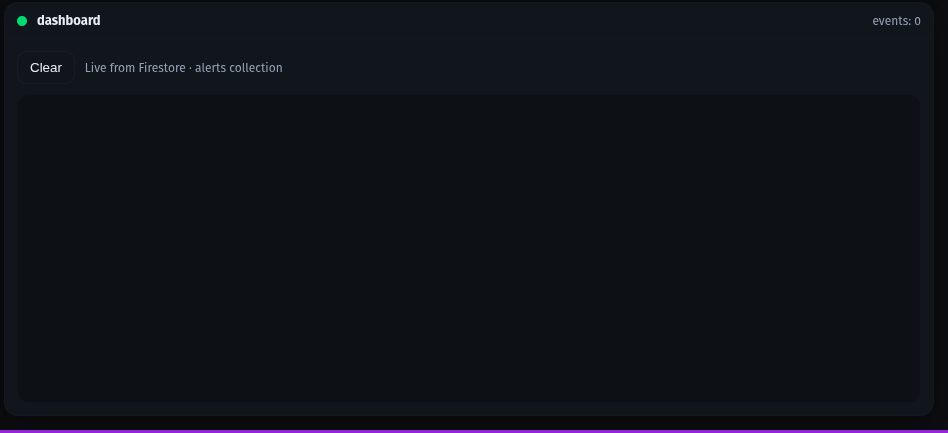
\includegraphics[width=\textwidth,keepaspectratio]{literature/dash_normal.png}\\[0.3em]
      {\small Normál állapot}
    \column{0.5\textwidth}
      \centering
      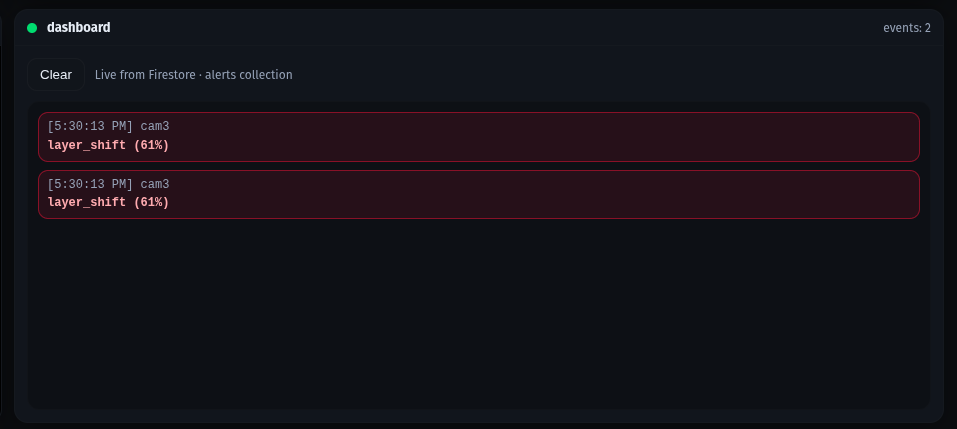
\includegraphics[width=\textwidth,keepaspectratio]{literature/dash_high.png}\\[0.3em]
      {\small\textcolor{alertred}{\textbf{Riasztás}} – piros keret}
  \end{columns}

  \vspace{0.35em}
  \centering
  {\footnotesize 3 élő WebRTC kamerastream + valós idejű detekciós napló (Firestore onSnapshot)}
\end{frame}

% ── Slide 13: Összefoglalás + Jövőbeli irányok ───────────────────────────────
\begin{frame}{Összefoglalás és jövőbeli irányok}
  \begin{columns}[T]
    \column{0.5\textwidth}
      \begin{block}{Elért eredmények}
        \begin{itemize}
          \setlength\itemsep{0.35em}
          \item 9 hibaosztály · mAP@0.5 = \textbf{0.892}
          \item Kétfázisú tanítás: csúcs \textbf{0.901}
          \item Teljes edge-cloud pipeline (Pi $\to$ GCP)
          \item Valós idejű dashboard + e-mail riasztás
          \item Terraform IaC + CI/CD automatizáció
        \end{itemize}
      \end{block}
    \column{0.5\textwidth}
      \begin{alertblock}{Jövőbeli irányok}
        \begin{itemize}
          \setlength\itemsep{0.35em}
          \item Konfidenciaküszöb szisztematikus hangolása
          \item Scale-to-zero (\$37/nap csökkentése)
          \item Aktív tanulási ciklus
          \item Nyomtatóvezérlő integráció (OctoPrint)
          \item Modell könnyűsúlyúsítása (YOLOv8n/s)
        \end{itemize}
      \end{alertblock}
  \end{columns}
\end{frame}

% ── Slide 14: Köszönet ────────────────────────────────────────────────────────
\begin{frame}[plain]
  \begin{beamercolorbox}[wd=\paperwidth,ht=2.2cm,dp=0pt,center]{frametitle}
    \vspace{0.6cm}
    {\Large\bfseries\color{white} Köszönöm a figyelmet!}
  \end{beamercolorbox}
  \vspace{1.4cm}
  \centering
  {\Large Kérdések?}

  \vspace{1.2em}
  {\small\color{primary}
    Borbáth Mátyás-Levente\\[0.3em]
    Sapientia Erdélyi Magyar Tudományegyetem, Marosvásárhely
  }\\[0.5em]
\end{frame}

\end{document}
